\section{Generaci\'on de Expresiones referenciales}

La generaci\'on de expresiones referenciales (GRE) {dado un contexto y un elemento
en ese contexto generar una expresi\'on gramaticalmente correcta en un lenguaje natural que representa \'unicamente el elemento {es una tarea b\'asica en lenguaje natural
generaci\'on, y una \'area de investigaci\'on activa (ver [4,5,6,20,8] entre otros). La mayor\'ia de
trabajo en esta \'area se centra en el problema de la determinaci\'on del contenido (es decir, encontrar una conjunto de propiedades que singulariza el objeto target de los restantes
objetos en el contexto) y deja la realizaci\'on real (es decir, que expresa un hecho
contenido como una expresi\'on gramaticalmente correcta) para tecnicas est\'andares.(excepto 16,21)
Sin embargo, a\'un no existe un acuerdo general sobre la representaci\'on b\'asica de
tanto la entrada y la salida del problema; esto se maneja m\'as bien de manera ad-hoc
por cada nueva propuesta.
Krahmer et al. [17] usan grafos dirigidos etiquetados en el contexto de este problema: los grafos son lo suficientemente abstractos para expresar un gran n\'umero de

dominios y hay muchos atractivos y algoritmos conocidos para tratar
con este tipo de estructuras. De hecho, no se trata de otra cosa que una representaci\'on alternativa de los modelos relacionales, usada t\'ipicamente para proporcionar sem\'antica a los lenguajes formales como el de primer orden y l\'ogicas de orden superior, l\'ogicas modales, etc.

''Incluso las valoraciones'' (esto no entendi...), los modelos b\'asicos de la l\'ogica proposicional, pueden ser vistos como un grafo de un solo punto etiquetado.
 No es de extra\~nar que son muy adecuadas para la tarea.
En este art\'iculo, nos ponemos del lado de [17] y usamos grafos etiquetados como entrada, pero sostenemos que una noci\'on importante se ha quedado fuera al tomar esta decisi\'on.


 Exactamente debido a su generalidad, los grafos no definen por s\'i mismos, una unica noci\'on de igualdad. �Cu\'ando decimos que dos nodos en el grafo pueden o no pueden ser
referenciados de forma \'unica en t\'erminos de sus propiedades? Esta pregunta s\'olo tiene sentido una vez que ya hemos fijado un cierto nivel de expresividad el cual determina cuando dos grafos, o dos elementos en el mismo gr\'afico, son equivalentes.
La expresividad se puede formalizar usando las relaciones estructurales de los grafos (iso
morfismos, etc.) o, alternativamente, lenguajes l\'ogicos. Ambas formas se presentan
en [cap2], donde tambi\'en discutimos c\'omo arreglar la noci\'on de impacto de expresividad en el n\'umero de casos que el problema GRE tiene soluci\'on; la complejidad computacional de los algoritmos GRE involucrados; y la complejidad computacional del problema de la realizaci\'on. Luego investigamos el problema GRE en t\'erminos de diferentes 
nociones de expresividad. Primero exploramos en [cap3] c\'omo algoritmos conocidos de
l\'ogica computacional se puede aplicar a GRE. Esta es una sistematizaci\'on de la aproximacion en [cita 1], y somos capaces de responder a la pregunta de complejidad que quedaba abierta.
En [cap4] tomamos el camino opuesto: tomamos el conocido algoritmo de GRE-
de [cita 17], identificamos su expresividad subyacente y lo reescribimos en t\'erminos de otras l\'ogicas.
A continuaci\'on, mostramos en [cap5] que ambos enfoques se pueden combinar y finalmente discutimos en [cap6] el tama\~no de una RE con respecto a la expresividad empleada. Llegamos a la conclusi\'on en [cap7] con una breve discusi\'on y las perspectivas para el trabajo futuro.

\newcommand{\nDog}{\mathit{dog}\xspace}
\newcommand{\nCat}{\mathit{cat}\xspace}
\newcommand{\aSmall}{\mathit{small}\xspace}
\newcommand{\aSniffing}{\mathit{sniffs}\xspace}
\newcommand{\nBreed}{\mathit{beagle}\xspace}

\section{Mediendo el poder expresivo}\label{sec:technical}


Las estructuras relacionales son muy adecuadas para la representaci\'on de situaciones o escenas. La estructura relacional (tambi\'en llamado ''el modelo relacional'') es un conjunto no vac\'io de objetos -el dominio- junto con una colecci\'on de las relaciones, cada uno con una aridad fija.
Formalmente, asumimos un vocabulario fijo y finito (pero arbitrario) vocabulario de
s\'imbolos de relaci\'on n-aria (las constantes y s\'imbolos de funciones pueden ser representadas como relaciones de aridad adecuada). 
Un modelo relacional $\+M$ es una tupla 
$\tup{\Delta,\interp{\cdot}}$ donde $\Delta$ es un conjunto no vac\'io, y
$\interp{\cdot}$ es una funci\'on de interpretaci\'on, esto es,
$\interp{r} \subseteq \Delta^n$ para todo s\'imbolo de relaci\'on $n$-aria tal que
$r$ est\'a en el vocabulario. Decimos que $\+M$ es \emph{finite} cuando
$\Delta$ es finito.  El \emph{tama\~no} de un modelo $\+M$ es la suma
$\#\Delta + \#\interp{\cdot}$, donde $\#\Delta$ es la cardinalidad
de $\Delta$ y $\#\interp{\cdot}$ es la suma de los tama\~nos de todas las
relaciones en $\interp{\cdot}$.

La Figura~\ref{fig:cat-dog-1} abajo muestra como nosotros podemos representar una escena
como un modelo relacional. Intuitivamente, $a$, $b$ y $d$ son dogs, mientras que 
$c$ y $e$ are cats;  $d$ es un small beagle;
 $b$ y $c$ son tambi\'en small.
 Nosotros leemos $\aSniffing(d,e)$ como ``{\em $d$ is sniffing $e$}''.

 \begin{figure}
 \begin{center}
 \begin{tabular}{rcl}
$\Delta$               & = & $\cset{a,b,c,d,e}$\\
$\interp{\nDog}$      & = & $\cset{a,b,d}$\\
$\interp{\nCat}$      & = & $\cset{c,e}$\\
$\interp{\nBreed}$    & = & $\cset{d}$\\
$\interp{\aSmall}$    & = & $\cset{b,c,d}$\\
$\interp{\aSniffing}$ & = & $\cset{(a,a),(b,a),(c,b),(d,e),(e,d)}$
 \end{tabular}
\begin{picture}(120,50)
\put(0,-50){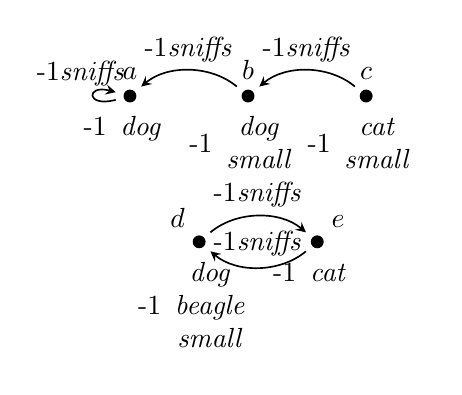
\begin{tikzpicture}
  [
    n/.style={circle,fill,draw,inner sep=1.5pt,node distance=1.5cm},
    aSniffing/.style={->, >=stealth, semithick, shorten <= 3pt, shorten >= 3pt},
  ]
 \node[n,label=above:$a$,label=below:{\relsize{-1}$\begin{array}{c}\nDog\end{array}$}] (a) {};

 \node[n,label=above:$b$,label=below:{\relsize{-1}$\begin{array}{c}\nDog\\ \aSmall \end{array}$}, right of=a] (b) {};

 \node[n,label=above:$c$,label=below:{\relsize{-1}$\begin{array}{c}\nCat\\ \aSmall\end{array}$}, right of=b] (c) {};

 \node[n,label=above left:$d$,label=below:{\relsize{-1}$\begin{array}{c}\nDog\\ \nBreed\\  \aSmall \end{array}$}, below of=a,xshift=25pt,yshift=-10pt] (d) {};

 \node[n,label=above right:$e$,,label=below:{\relsize{-1}$\begin{array}{c}\nCat\end{array}$},right of=d] (e) {};

 \draw [aSniffing,loop left] (a) to node[above,xshift=-5pt]{\relsize{-1}$\aSniffing$} (a);

 \draw [aSniffing,bend right=40] (b) to node[auto,swap]{\relsize{-1}$\aSniffing$} (a);

 \draw [aSniffing,bend right=40] (c) to node[auto,swap]{\relsize{-1}$\aSniffing$} (b);

 \draw[aSniffing, bend left=40] (d) to node[auto]{\relsize{-1}$\aSniffing$} (e);
 \draw[aSniffing, bend left=40] (e) to node[auto,swap]{\relsize{-1}$\aSniffing$} (d);

 \end{tikzpicture}}
 \end{picture}

 \end{center}
 \caption{Representaci\'on de escenas de Graph $\+S$.\label{fig:cat-dog-1}}
 \end{figure}


Los languajes logicos son \'utiles para la tarea (formalmente) \emph{describiendo}
elementos de una estructura relational. Consider, por ejemplo, el lenguaje clasico
de l\'ogica de primer-orden (con igualdad), \FOL, dado por:
$$
  \top \mid x_i \not\approx x_j \mid  r (\bar x) \mid \lnot \gamma \mid \gamma \land \gamma' \mid \exists x_i . \gamma
$$
%
donde $\gamma,\gamma' \in \FOL$,
$r$ es un s\'imbolo de relaci\'on $n$-ario y $\bar x$ es un $n$-tuple de variables.
Como es usual, $\gamma \lor \gamma'$ y $\forall x . \gamma$ son las versiones cortas de
$\lnot(\lnot\gamma \land \lnot\gamma')$ y $\lnot\exists x . \lnot\gamma$, respectivamente.
Formulas of the form $\top$, $x_i \not\approx x_j$ and $r(\bar
x)$ son llamados \emph{atomos}.%
  \footnote{%
    Por razones t\'ecnicas, incluimos el s\'imbolo de desigualdad symbol $\not \approx$ como
    primitivo.  Igualdad puede ser definido usando negaci\'on.
  }
Dado un modelo relacional $\+M = \tup{\Delta,\interp{\cdot}}$ y una
f\'ormula $\gamma$ con variables libres%
\footnote{%
    W.l.o.g.\ asumimos que no aparecen variable en ambos, libres y ligadas, que una variable no esta ligada 2 veces,
    y que el \'indice de las variables crece en la f\'ormula de izquierda a derecha.%
}
entre $x_1\ldots x_n$, inductivamente definimos la \emph{extensi\'on} o
\emph{interpretaci\'on} de $\gamma$ como el conjunto de $n$-tuplas
 $\interp{\gamma}^n \subseteq \Delta^n$ que satisface:

\begin{center}
\begin{tabular}{rcl@{\hspace{1cm}}rcl}
$\interp{\top}^n$ &$=$& $\Delta^n$
&
$\interp{x_i \not\approx x_j}^n$ &$=$& $\cset{\bar{a} \mid \bar{a} \,{\in}\, \Delta^n, a_i \neq a_j}$
\\
$\interp{\lnot\delta}^n$ &$=$& $\Delta^n \setminus \interp{\delta}^n$
&
$\interp{r (x_{i_1} \ldots x_{i_k})}^n$ & $=$&$\cset{\bar{a} \mid \bar{a} \,{\in}\, \Delta^n, (a_{i_1} \ldots a_{i_k}) {\in} \interp{r}}$
\\
$\interp{\delta \land \theta}^n$ &$=$& $\interp{\delta}^n \cap \interp{\theta}^n$
&
$\interp{\exists x_{l}.\delta}^n$ &$=$& $\cset{\bar a \mid \bar a  e  \in \interp{\delta'}^{n+1}\ \text{for some $e$}}$
\end{tabular}
\end{center}
%
donde $1 \le i,j, i_1, \ldots, i_k \le n$, $\bar{a} = (a_1\ldots
a_n)$, $\bar{a}e = (a_1\ldots a_n,e)$ y $\delta'$ son
obtenidos reeplazando todas las ocurrencias de $x_l$ en $\delta$ por
$x_{n+1}$. Cuando la cardinalidad de las tuplas involucradas en el contexto es conocida 
escribiremos $\interp{\gamma}$ en lugar de
$\interp{\gamma}^n$.

Con una sintaxis y sem\'antica de un lenguaje en mente, podemos formalmente definir el problema de L-GRE para un conjunto target de elementos T (lejeramente adaptaremos la definici\'on en ~\cite{AKS08}):

\medskip
\noindent
{\small
\begin{center}
\begin{tabular}{ll} \hline
\multicolumn{2}{l}{
\textsc{Problema $\gL$-GRE }}\\ \hline
\ \ Input: & a model $\gM=\tup{\Delta,\interp{\cdot}}$ and a nonempty target  set $T \subseteq \Delta$.\\
\ \ Output: & a formula $\varphi \in \gL$ such that
$\interp{\varphi} = T$ if it exists, and $\bot$ otherwise.\\ \hline
\end{tabular}
\end{center}}
Cuando el output es no $\bot$, decimos que $\phi$ es una
\emph{$\+L$-referring expression ($\+L$-RE) para $T$ en $\+M$}.
Simply put then, el output de el problema $\+L$-GRE es una f\'ormula de
$\+L$ cuya interpretaci\'on en el modelo de input es el conjunto target, si
tal f\'ormula existe.  Esta definici\'on aplica incluso a la GRE para
objetos  de el dominio teniendo un conjunto singleton como target.

Mediante el uso de f\'ormulas con n variables libres se podr\'ia extender esta defici\'on para
describir relaciones n-arias; pero aqu\'i s\'olo estamos interesados ??en la descripci\'on de subconjuntos de
el dominio. En realidad, limitaremos nuestra atenci\'on un poco m\'as:
Convenci\'on 1. S\'olo consideraremos modelos relacionales con s\'imbolos de relaciones unarias y binarias
 (es decir, grafos etiquetados ). Usaremos p para los s\'imbolo de relaci\'on unarios
 (y lo llamaremos una proposici\'on) y r para los s\'imbolos de relaciones binarios.
Esta convenci\'on captura los modelos habituales de inter\'es al describir escenas como
el presentado en la Figura ~\ref{fig:cat-dog-1}. Acomodando las relaciones de mayor aridad en nuestra
marco te\'orico es f\'acil, pero puede ser que una complejidad computacional? ect.

\subsection{Elecci\'on del lenguaje apropiado}\label{sec:choosinglanguage}

Dado un modelo M, podr\'ia haber un infinito n\'umero de f\'ormulas que de forma \'unica
describan un target (incluso f\'ormulas que no son l\'ogicamente equivalentes podr\'ian tener
la misma interpretaci\'on una vez al modelo este fijo). A pesar de tener la misma interpretaci\'on en M, ellos pueden ser muy diferentes con respecto a otros par\'ametros.
Como es bien conocido en la comunidad generaci\'on de texto automatizado, diferentes
realizaciones del mismo contenido podr\'ian dar lugar a expresiones referenciales que son m\'as o menos
apropiadas en el contexto dado. Aunque, como hemos mencionado en la introducci\'on,
s\'olo nos ocuparemos de la parte determinaci\'on del contenido (y no de la parte de realizaci\'on) del problema GRE, argumentamos que la generaci\'on de contenido usando lenguajes con diferente poder expresivo puede tener un impacto en la estapa posterior
de generaci\'on de superficie (surface realization, realizaci\'on sint\'actica... pero es mucho m\'as que eso... ).


Consideremos de nuevo la escena en la Figura~\ref{fig:cat-dog-1}. F\'ormulas

$\gamma_1$--$\gamma_4$ mostradas en la Tabla~\ref{tab:gammas}
son todas de tal manera que $\gamma_i$ \'unicamente describe a $b$
(es decir, $\interp{\gamma_i} = \cset{b}$) en el modelo $\+S$.
Podr\'ia decirse que, $\gamma_1$ puede ser f\'acilmente realizada como \emph{``the small dog
that sniffs a dog''}. Sint\'acticamente, $\gamma_1$ es caracterizada como una f\'ormula positiva, conjuntiva, existencial (es decir, no contiene negaci\'on y s\'olo utiliza la conjunci\'on y cuantificaci\'on existencial). Expresiones
con estas caracter\'isticas son, por mucho, las m\'as encontradas en los corpus de ER
como los recopilados en~\cite{viet:algo06,deem:buil06,dale:refe09}. La f\'ormula $\gamma_2$, por otro lado, contiene negaci\'on,
disyunci\'on y cuantificaci\'on universal. Podr\'ia realizarse como \emph{``the small dog that
only sniffs things that are not cats''} lo cual suena poco natural. 

Incluso un peque\~no cambio en la f\'ormula $\gamma_2$ la hace m\'as aceptable:
reescribirla usando $\exists$, $\lnot$, y $\land$ para obtener
\emph{``the small dog that is not sniffing a cat''}. Similarmente,
 $\gamma_3$ y $\gamma_4$ son computacionalmente m\'as dificiles de realizar que 
 $\gamma_1$: $\gamma_3$ contiene desigualdad (\emph{``the dog sniffing another dog''}), mientras que el objeto cuantificado aparece en posici\'on del primer argumento en la relaci\'on binaria en $\gamma_4$ (\emph{``the dog that is sniffed by a small cat''}).


Resumiendo, podemos asegurar, ya durante la fase de determinaci\'on de contenido,
ciertas propiedades de la expresi\'on referencial generada prestando atenci\'on a
el lenguaje formal utilizado en la representaci\'on. Y podemos hacer esto, incluso antes
teniendo en cuenta otros aspectos ling�\'isticos fundamentales que se asegurar\'a de
realizaci\'on preferible, como la prominencia, la capacidad cognitiva del oyente (puede que
reconocer un beagle de otro tipo de perro?), etc.
Como ejemplo concreto, sea FO- ser el fragmento del FO-f\'ormulas donde el operador negacion no ocurre (pero note que xi distinto de xj esta permitido)
 
\begin{table}
$$
\begin{array}{cl}
 \gamma_1: & \nDog(x) \land \aSmall(x) \land
   \exists y . (\aSniffing(x,y) \land \nDog(y))\\[3pt]
  %
  \gamma_2: & \nDog(x) \land \aSmall(x) \land
  \forall y . (\neg \nCat(y) \lor \neg \aSniffing(x,y))\\[3pt]
  %
  \gamma_3: & \nDog(x) \land
  \exists y . (x \not\approx y \land \nDog(y)  \land \aSniffing(x,y))\\[3pt]
  %
  \gamma_4: & \nDog(x) \land
  \exists y . (\nCat(y) \land \aSmall(y) \land \aSniffing(y,x))
  %
 \end{array}
$$
\caption{Descripciones alternativas para el objeto $b$ en el modelo mostrado en Figura~\ref{fig:cat-dog-1}.}\label{tab:gammas}
\end{table}

Restringiendo la determinaci\'on de contenido a FO-, aseguramos que f\'ormulas como  $\gamma_2$ no se generar\'an. Si prohibimos el distinto del lenguaje  $\gamma_3$ tambi\'en queda exclu\'ida.

El hecho de que el lenguaje de representaci\'on utilizado tiene un impacto sobre la determinaci\'on de contenido es obvio, pero no ha recibido la atenci\'on que merece. Areces et al. [1] usaron diferentes l\'ogicas de descripci\'on (una familia de lenguajes formales utilizado en representaci\'on del conocimiento, vea [2]) para clasificar y dar un marco formal para
trabajo previo sobre GRE. Vamos a presentar r\'apidamente algunas de estos lenguajes ya que los mencionaremos en las siguientes secciones. Usando l\'ogicas de descripci\'on en lugar de fragmentos de FO es s\'olo una cuesti\'on de notaci\'on, como la mayor\'ia de l\'ogicas descriptivas se pueden ver
fragmentos como impl\'icitas de FO. Por ejemplo, el lenguaje de la l\'ogica de descripci\'on ALC, se define sint\'acticamente como el conjunto de f\'ormulas,
$$
\top \mid p \mid \neg \gamma \mid \gamma \wedge \gamma' \mid  \exists r. \gamma
$$
(donde $p$ es un s\'imbolo proposicional, $r$ s\'imbolo relacional binario, y $\gamma,\gamma' \in \ALC$) corresponde al fragmento sint\'actico de
\FOL sin $\not\approx$, como es mostrado por la traducci\'on est\'andar $\st_x$:

\begin{center}
\begin{tabular}{rcl@{\hspace{1cm}}rcl}
$ \st_{x_i}(\top)$ &$=$& $\top$
&
$\st_{x_i}(\gamma_1 \land \gamma_2)$ &$=$& $\st_{x_i}(\gamma_1) \land \st_{x_i}(\gamma_2)$
\\
  $\st_{x_i}(p)$ &$=$& $p(x_i)$
&
$\st_{x_i}(\exists r . \gamma)$ &$=$& $\exists x_{i+1} . (r(x_i,x_{i+1}) \land \st_{x_{i+1}}(\gamma))$
\\
 $\st_{x_i}(\lnot \gamma)$ &$=$& $\lnot\st_{x_i}(\gamma)$
&
\end{tabular}
\end{center}

En efecto, dado un modelo relacional $\+M$, la extensi\'on de una f\'ormula \ALC en M coincide exactamente con la extensi\'on de $\st_{x_1}(\varphi)$ (v\'ease, por ejemplo, ~\cite{baad:desc03}). Gracias
a este resultado, para cualquier f\'ormula $\varphi$ de \ALC y sus sublenguajes podemos definir $\interp{\varphi} = \interp{\st_{x_1}(\varphi)}$.
 Volviendo a nuestro ejemplo anterior, mediante la restricci\'on de contenido
generaci\'on en f\'ormulas $\ALC$ (o equivalentemente, el fragmento correspondiente de \FOL)
evitar\'iamos f\'ormulas como
$\gamma_3$ (sin igualdad) y
$\gamma_4$ (aparece cuanti elemento ed
siempre en segunda posici\'on de argumento).
Generaci\'on se discute en ~\cite{AKS08}, en t\'erminos de diferentes l\'ogicas de descripci\'on como \ALC
y \EL (\ALC sin negaci\'on). Vamos a ampliar los resultados en ese papel, con-
Sidering por ejemplo \ELAN (\ALC con la negaci\'on permitida s\'olo frente a relaciones unarias), pero, en general, nosotros tomamos un enfoque modelo te\'orico y argumentamos que la cuesti\'on principal no es si se debe utilizar una u otra (descripci\'on l\'ogica para la generaci\'on de contenido, sino que son el diferencias sem\'antica a tener en cuenta. Esto no solo determina el formalismo l\'ogico requerido sino tambi\'en impacta tanto en la determinaci\'on de contenido como en los problemas de realizaci\'on sint\'actica. Cada
lenguaje l\'ogico puede ser visto como un compromiso entre la expresividad, realizabilidad y complejidad computacional. La selecci\'on apropiada para una tarea GRE particular, debe depender del contexto actual


\subsection{Definiendo \emph{Similaridad}}

Intuitivamente, dado un lenguaje l\'ogico $\+L$ decimos que un objeto $u$ en un modelo
$\+M_1$ es similar en $\+L$ a otro objeto
 $v$ en el model $\+M_2$ para cualquier $\+L$-formulas que son satisfechas por $u$ tambi\'en son satisfechasa por $v$. Formalmente,
%let $\+L$ stand for any of the languages discussed so far, and
Sea $\+M_1 = \tup{\Delta_1, \interp{\cdot}_1}$ y $\+M_2 = \tup{\Delta_2, \interp{\cdot}_2}$ ser 2 modelos relacionales con $u \in \Delta_1$ y $v \in \Delta_2$; seguimos la terminolog\'ia de~\cite{AKS08} y decimos que
\emph{$u$ es $\+L$-similar a $v$}  (notaci\'on $u \simil{\+L} v$) cualquier $u \in \interp{\gamma}_1$ implica
$v \in \interp{\gamma}_2$, para toda $\gamma \in \+L$. Es facil mostrar que
$\+L$-similaridad es reflexiva para todo $\+L$, y simm\'etrica  para languajes que contienen negaci\'on.


Observe que la $\+L$-similitud captura la noci\'on de `capacidad de identificar en $\+L$'. Si tomamos $\+M_1$ y $\+M_2$ a ser del mismo modelo, un objeto $u$ en el modelo identificarse un\'ivocamente en $\+L$ si no hay ning\'un objeto $v$ diferente de $u$ tal que $u \simil{\+L} v$. En otras palabras, si hay dos objetos $u$ y $v$ en un modelo M tal que
$u \simil{\+L} v$, entonces el problema $\+L$-GRE con entrada de $\+M$ y destino $T=\{u\}$ no tendr\'a \'exito ya que para todas las f\'ormulas $\gamma \in L$ tenemos que $\{u,v\} \subseteq \interp{\gamma} \not = \{u\}$.

La noci\'on de $\+L$-similitud entonces, nos permite manejar el problema de  $\+L$-GRE.
Por otra parte, podemos reformular esta de noci\'on de una manera estructural, por lo que no lo hacemos
que considerar en muchos $\+L$-f\'ormulas infinitamente decidir si $u$ es $\+L$- similar a $v$. Podemos reinterpretar $\+L$-similitud en t\'erminos de nociones de teor\'ia de modelos estandares
como isomorfismos o bisimulationes que describen las propiedades estructurales del modelo. Dados dos modelos$\tup{\Delta_1, \interp{\cdot}_1}$ and $\tup{\Delta_2,
\interp{\cdot}_2}$, considere las siguiente
propiedades de una relaci\'on binaria ${\sim} \subseteq \Delta_1 \times \Delta_2$ (cf.~Convention~\ref{conv:signature}):
\smallskip 

\newcommand{\simdef}[2]{\noindent\ \ #1\hfill:\ \parbox[t]{.87\textwidth}{#2}\par}

\simdef{$\atomL$}{If $u_1{\sim} u_2$, entonces $u_1 \in \interp{p}_1 \Rightarrow u_2 \in \interp{p}_2$}
\simdef{$\atomR$}{If $u_1{\sim} u_2$, entonces $u_2 \in \interp{p}_2 \Rightarrow u_1 \in \interp{p}_1$}
\simdef{$\zig$}{If $u_1{\sim} u_2$ y $(u_1,v_1) \in \interp{r}_1$, entonces $\exists v_2$ s.t.\ $v_1{\sim}v_2$
  y $(u_2,v_2) \in \interp{r}_2$}
\simdef{$\zag$}{If $u_1{\sim}u_2$ y $(u_2,v_2) \in \interp{r}_2$, entonces $\exists v_1$ s.t.\ $u_1{\sim}v_1$ y
 $(u_1,v_1) \in \interp{r}_1$}
\simdef{$\injL$}{$\sim$ es una funci\'on inyectiva (cuando es restringida a su dominio)}
\simdef{$\injR$}{$\sim^{-1}$ es una funci\'on inyectiva (cuando es restringida a su dominio)}
\smallskip

Diremos que una relacion binaria no-vac\'ia $\sim$ es una 
\emph{$\+L$-simulation} cuando satisface las propiedades indicadas
en la Tabla~\ref{tab:simuls}. Por ejemplo, una relacion binaria no-vac\'ia que satisface $\atomL$, y $\zig$ es una $\EL$-simulation, como es indicado en fila~4 de la Tabla~\ref{tab:simuls}. M\'as a\'un, diremos que un objeto
\emph{$v$ $\+L$-simulates $u$} (notaci\'on $u \simul{\+L} v$) si hay una relaci\'on $\sim$ que satisface el correspondite propiedad tal que
$u \sim v$. El siguiente es un resultado fundamentar del modelo-teor\'etico  result:%~\cite{ebbi:math96,KR99,BRV01}

\begin{table}[t]
$$
\begin{array}{c|cccccc}
  \+L & \atomL & \atomR & \zig & \zag & \injL & \injR \\
  \hline
  \FOL   & \times & \times & \times & \times & \times & \times\\
  \EPFOL & \times & & \times && \times &\\
  \ALC   & \times & \times & \times & \times&&\\
  \EL    & \times & &  \times & &\\
  \ELAN  & \times & \times &  \times & &\\
\end{array}
$$
\caption{$\+L$-simulations for several logical languages $\+L$.}\label{tab:simuls}
\end{table}

\begin{theorem} \label{thm:simulation}
If  $\+M_1 = \tup{\Delta_1, \interp{\cdot}_1}$ and $\+M_2 =
\tup{\Delta_2, \interp{\cdot}_2}$ son modelos finitos, $u \in
\Delta_1$ and $v \in \Delta_2$, then $u \simil{\+L} v$ iff $u
\simul{\+L} v$ (for $\+L \in \cset{\FOL,\EPFOL,\ALC,\EL,\ELAN}$).
\end{theorem}
\begin{proof}
Algunos resultados son bien conocidos: $\simul{\FOL}$ es isomorfismo en
grafos etiquetados~\cite{ebbi:math96}; $\simul{\ALC}$ corresponde a la
noci\'on de bisimulaci\'on~\cite[Def.~2.16]{BRV01}; $\simul{\EL}$ es una
simulaci\'on definida en~\cite[Def.~2.77]{BRV01}. Los restantes son variaciones de estos.
\end{proof}


Therefore, on finite models\footnote{Finiteness is not the weakest hypothesis,
but it is enough for our development.} simulations capture exactly the notion of similarity.
The right to left implication does not hold in general on infinite
models.

$\+L$-simulations allow us to determine, in an effective way,
when an object is indistinguishable from another in a given model with respect to $\+L$.

For example, we can verify that $a \simul{\EL} b$ in the model of
Figure~\ref{fig:cat-dog-1} (the relation ${\sim} = \{(a,a), (a, b) \}
%\cup\{ (x,x) \mid x \in \Delta\}
$ satisfies $\atomL$ and $\zig$).
Using Theorem~\ref{thm:simulation}
we conclude that there is no \EL-description for $a$, since for any \EL-formula $\gamma$,
if $a\in\interp{\gamma}$, then $b\in\interp{\gamma}$.
Observe that $b \not\simul{\EL} a$, since
(again applying Theorem~\ref{thm:simulation}), $b\in\interp{\aSmall(x)}$ but
$a\notin\interp{\aSmall(x)}$.
%
If one chooses a language richer than $\EL$, such as $\ELAN$, one may be
able to describe $a$: take, for instance the $\ELAN$-formula
$\nDog(x)\wedge\lnot\aSmall(x)$.


As we will discuss in the next section, simulation gives us an
efficient, computationally feasible approach to the $\+L$-GRE
problem. Algorithms to compute many kinds of $\+L$-simulations are
well known (see, \cite{H71,PT87,HHK95,DPP03}), and for many
languages  (e.g., \ALC, \ALC with inverse relations,  \ELAN and \EL)
they run in polynomial time (on the other hand, no polynomial
algorithm for \FOL- or \EPFOL-simulation is known and even the exact
complexity of the problem in these cases is open
\cite{gare:comp79}).

\section{GRE via Simulator Sets}\label{sec:simulation}

En esta secci\'on discutiremos como resolver el problema $\+L$-GRE
usando simulation. Dado a model $\+M = \tup{\Delta,
\interp{\cdot}}$, Theorema~\ref{thm:simulation} nos dice que si 2 elementos distintos $u$ y $v$ en $\Delta$ son tales que $u
\simul{\+L} v$ entonces para toda $\+L$-f\'ormula que es verdadera para $u$ es tambi\'en verdadera para $v$. No hay f\'ormula en $\+L$ que pueda identificar un\'ivocamente a $u$. Desde esta perspectiva, conociendo cuando el modelo contiene un elemento que es $\gL$-similar pero distinto de $u$ es
equivalente a decidir hay una $\+L$-RE for $u$.


Asumamos un lenguaje fixo $\+L$ y un modelo $\+M$.  Supongamos que queremos referirnos a un elemento $u$ del dominio de $\+M$. Queremos computar \emph{simulator set} de $u$ definidas como
$\simset_{\+L}^{\+M}(u) = \cset{v \in \Delta \mid u \simul{\+L} v}$.
Cuando un modelo $\+M$ is clear from the context, we just write
$\simset_{\+L}$.
 If $\simset_{\+L}^{\+M}(u)$ no es singleton $\cset{u}$,
el problem $\+L$-GRE con target $\{u\}$ en $\+M$ fallar\'a.

\iffullversion
Es facil de ver que la union de 2 $\+L$-simulations es
es tambi\'en una $\+L$-simulation. Podemos entonces definir el \emph{maximal
auto $\+L$-simulation} (notaci\'on, $\simmax_{\+L}$) sobre un modelo $\+M$ como la union de todos los
auto $\+L$-simulations sobre $\+M$. Ya que
$\simset_{\+L}(u) = \cset{v \mid u \simmax_{\+L} v}$, un algoritmo
para computar $\simmax_{\+L}$ tambi\'en computa $\simset_{\+L}(u)$.
\else
\fi

\iffullversion
If $P$ es reflexiva y transitiva entonces tambi\'en lo es $\simmax_P$. En
particular, $\simmax$ es reflexiva y transitiva.
\fixme{Are reflexivity and transitivity important? Check.}
\else
\fi



Un algoritmo es dado en~\cite{HHK95} para computar $\simset_{\ELAN}(v)$ para cada
elemento $v$ de un modelo dado finito
$\+M=\tup{\Delta,\interp{\cdot}}$
%\footnote{%
%  Actually the algorithm proposed in \cite{HHK95} is over labeled graphs, but
%  it can be adapted to compute $\simset_{\ELAN}$ by
%  appropriately labeling the model.%
%}
en tiempo $O(\size{\Delta}\times\size{{\interp{\cdot}}})$.
Intuitivamente, este algoritmo
define $S(v)$ como un conjunto de candidatos para simuolar $v$ y
sucesivamente refina este borrando aquellos los cuales falla en simular $v$.
%Since we never put new vertices into $\simset(v)$, all the deletions
%from $\simset(v)$ are permanent.
Al final, $S(v)=\simset_\ELAN(v)$. El algoritmo puede ser adaptado para
computar $\simset_\+L$ para cualquier otro languaje $\+L$. En particular,
lo podemos usar para computar $\simset_\EL$ en tiempo polinomial which will
give us the basic algorithm for establishing an upper bound to the
complexity of the \EL-GRE problem --this will answer an open
question of~\cite{AKS08}. The pseudo-code is shown in
Algorithm~\ref{alg:schematic-gen-sim}, which uses the following
notation: $\+P$ is a fixed set of unary relation symbols,  for $v\in
\Delta$, let $\unary(v)=\{p\in\+P\mid v\in\interp{p}\}$ and let also
$\su{r}{v}=\{u\in\Delta\mid(v,u)\in\interp{r}\}$ for $r$ a binary
relation symbol.

\begin{algorithm} \small
\caption{\small Computing \EL-similarity}\label{alg:schematic-gen-sim}
\SetKwInOut{Input}{input}\SetKwInOut{Output}{output}
\Input{a finite model $\+M=\tup{\Delta,\interp{\cdot}}$}
\Output{$\forall v\in \Delta$, the simulator set
$\simset_\EL^{\+M}(v)=S(v)$} \BlankLine

\ForEach{$v\in \Delta$}{$S(v):=\{u\in \Delta \mid \unary(v)
\subseteq \unary(u) \}$}

\While{\guard}{$S(u):=S(u)\setminus\{w\}$}
\end{algorithm}


%First some notation. For any $v\in \Delta$ and any binary relation
%$r$, let
%\begin{eqnarray*}
%\unary(v)&=&\{p\mid \mbox{$p$ is a unary rel.\ and
%$v\in\interp{p}$}\}\\
%%\pr{r}{v}&=&\{u\in\Delta\mid(u,v)\in\interp{r}\}\\
%\su{r}{v}&=&\{u\in\Delta\mid(v,u)\in\interp{r}\}
%\end{eqnarray*}
%%The last two extend to sets $V\subseteq\Delta$ as usual:
%%$\pr{r}{V}=\bigcup_{v\in V}\pr{r}{v}$ and $\su{r}{V}=\bigcup_{v\in
%%V}\su{r}{v}$.

%

The algorithm is fairly straightforward. We initialize $S(v)$ with
the set of all elements $u\in\Delta$ such that $\unary(v)\subseteq
\unary(u)$, i.e., the set of all elements satisfying at least the
same unary relations as $v$ (this guarantees that property $\atomL$ holds).
At each step, if there are three elements $u$, $v$ and $w$ such that
for some relation $r$, $(u,v) \in \interp{r}$, $w\in S(u)$
(i.e., $w$ is a candidate to simulate $u$) but $\su{r}{w}\cap S(v) = \emptyset$
(there is no element $w'$ such that $(w, w') \in \interp{r}$
and $w'\in S(v)$) then clearly condition $\zig$ is not satisfied
under the supposition that $\simset_\EL=S$. $S$ is `too big' because
$w$ cannot simulate $u$. Hence $w$ is removed from $S(u)$.

Algorithm~\ref{alg:schematic-gen-sim} will only tell us
whether an \EL-RE for an element $u$ exists (that is,
whether $\simset_{\EL}(u) = \cset{u}$ or not).  It does not compute
an \EL-formula $\varphi$ that uniquely refers to $v$. But
we can adapt it to obtain such a formula.
Algorithm~\ref{alg:schematic-gen-sim}'s main strategy to compute simulations
is to successively
refine an over-approximation of the simulator sets.
The ``reason'' behind each refinement  can be encoded using an \EL-formula.
Using this insight, one can transform an algorithm that computes
$\+L$-simulator sets with a similar strategy,  into one that additionally computes an $\+L$-RE
for each set.


Algorithm~\ref{alg:schematic-GRE} shows a transformed version of
Algorithm~\ref{alg:schematic-gen-sim} following this principle. The
idea is that each node $v\in\Delta$ is now tagged with a formula
$F(v)$ of \EL. The formulas $F(v)$ are updated along the execution of
the loop, whose invariant  ensures that $v \in
\interp{F(v)}$ and $\interp{F(u)} \subseteq S(u)$ hold for all
$u,v\in\Delta$.

\begin{algorithm}\small
%\LinesNumbered
\io

\ForEach{$v\in \Delta$}{ $S(v):=\{u\in \Delta \mid \unary(v)
\subseteq \unary(u) \}$\;\label{alg:line:init1}

$F(v):=\bigwedge \unary(v)$\;\label{alg:line:init2} }

\While{\guard}
{
 %$\{\ I: \mbox{\bf assert }(\forall u,v)\ \interp{F(u)} \subseteq S(u)\wedge v \in \interp{F(v)} \ \}$
 \KwSty{invariant} $\forall u,v: \interp{F(u)} \subseteq S(u)\wedge v \in \interp{F(v)}$\\
$S(u):=S(u)\setminus\{w\}$\;\label{alg:line:loop-body-begin}

\If{$\diam F(v)$ is not a conjunct of $F(u)$}{ $F(u):=F(u)\wedge
\diam F(v)$\;\label{alg:line:loop-body-end-1} }} \caption{\small
Computing $\EL$-similarity and \posre}\label{alg:schematic-GRE}
\end{algorithm}

Initially $F(v)$ is the conjunction of all the unary relations that
satisfy $v$ (if there is none, then $F(v)=\top$).
Each time the algorithm finds elements $r,u,v,w$
such that $(u,v)\in\interp{r}$, $w\in S(u)$ and $\su{r}{w}\cap
S(v)=\emptyset$, it updates $F(u)$ to $F(u)\wedge\diam F(v)$.
Again this new formula $\phi$ is in $\pos$ and it can be
shown that $v\in\interp{\phi}$ and $w\notin\interp{\phi}$, hence
witnessing that $v\simil{\EL} w$ is false.

%As we will see in Theorem~\ref{thm:correctness-schematic-GRE}, this
%formula is true in $v$ but false in $w$, hence witnessing that $w$
%does not simulate $v$.


%It is clear that Algorithm \ref{alg:schematic-GRE} terminates.

\iffullversion One wants to know whether a given set $V\subseteq W$
has an \posre. How do we interpret the output of Algorithm
\ref{alg:schematic-GRE}? Here is the answer: $V\subseteq W$ has an
\EL-RE iff there is a node $v\in V$ such that $V=\{u\in W\colon
v\in\simset_\subseteq(u) \wedge u\in\simset_\subseteq(v)\}$. In
other words, $V$ has an \EL-RE iff $V$ is the set of nodes which are
\emph{bisimilar} to some node of $V$. Here we say that $u$ and $v$
are \emph{bisimilar} if $u\in\simset_\subseteq(v)$ and
$v\in\simset_\subseteq(u)$. In case $V=\{v_1,\dots,v_n\}$ has an
\posre, any $F(v_i)$ is a valid \posre, so one can pick any of them.

In particular, $v$ has an \EL-RE if and only if $\simset_\subseteq(v)=\{v\}$
and in case $v$ has a \EL-referring expression then $F(v)$ is a
valid one. If $v$ does not have an \posre then the algorithm may be
used to approximate an \posre. Indeed, since every formula true at
$v$ is also true at all nodes in $\simset_\subseteq(v)$ and $F(v)$
is true at every node of $\simset_\subseteq(v)$ then $F(v)$ is a
reasonable approximation of an \EL-RE for $v$.

\begin{ex}
Let $\gG$ be the following model
\begin{center}
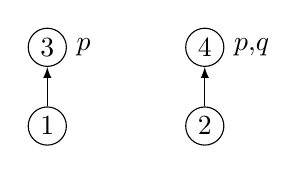
\begin{tikzpicture}[>=latex]
  \node (n1) at (0,0) [shape=circle,draw,inner sep=2pt, label=right:$$] {$1$} ;
  \node (n2) at (2,0) [shape=circle,draw,inner sep=2pt, label=right:$$] {$2$} ;
  \node (n4) at (0,1) [shape=circle,draw,inner sep=2pt, label=right:$p$] {$3$} ;
  \node (n5) at (2,1) [shape=circle,draw,inner sep=2pt, label=right:$p{,}q$] {$4$} ;
  \draw [->] (n1) -- (n4);
  \draw [->] (n2) -- (n5);
\end{tikzpicture}
\end{center}
%
where $\rg\ l=\cset{p,q}$ and the valuation is defined as
$l(3)=\cset{p}, l(4)=\cset{p,q}, l(1)=l(2)=\cset{}$. The initial values of $S$ and $F$ are
shown in Table~\ref{tab:example}.

\begin{table}[ht]
\centering
{\footnotesize
\begin{tabular}{|c|c|c|c|c|}
\hline
&\multicolumn{2}{|c|}{Initial}&\multicolumn{2}{|c|}{Final}\\
$v$ & $S(v)$ & $F(v)$ & $S(v)$&$F(v)$\\
\hline
$1$ & $\{1,2,3,4\}$ & $\top$ & $\{1,2\}$&$\top\wedge\diam p$\\
$2$ & $\{1,2,3,4\}$ & $\top$ & $\{2\}$&$\top\wedge\diam(p\wedge q)$\\
$3$ & $\{3,4\}$ & $p$ & $\{3,4\}$ &$p$\\
$4$ & $\{4\}$ & $p\wedge q$ & $\{4\}$&$p\wedge q$\\
\hline
\end{tabular}
\caption{Initial and final values of $F$ and $S$}\label{tab:example}
}
\end{table}

Suppose the following execution:
\begin{enumerate}
\item Choose $u=2,v=4,w=1$: detect that $1$ does not simulate $2$; set $S(2)=\{2,3,4\}$ and $F(2)=\top\wedge\diam(p\wedge q)$
\item Choose $u=2,v=4,w=3$: detect that $3$ does not simulate $2$; set $S(2)=\{2,4\}$ and $F(2)=\top\wedge\diam(p\wedge q)$
\item Choose $u=2,v=4,w=4$: detect that $4$ does not simulate $2$; set $S(2)=\{2\}$ and $F(2)=\top\wedge\diam(p\wedge q)$
\item Choose $u=1,v=3,w=3$: detect that $3$ does not simulate $1$; set $S(1)=\{1,2,4\}$ and $F(1)=\top\wedge\diam p$
\item Choose $u=1,v=3,w=4$: detect that $4$ does not simulate $1$; set $S(1)=\{1,2\}$ and $F(1)=\top\wedge\diam p$
\end{enumerate}
After the fifth iteration it terminates. The final output is shown
in Table~\ref{tab:example}. From this output one may conclude that,
since $\simset_\subseteq(4)=\{4\}$, node $4$ has an \posre, namely
$p\wedge q$. Node $2$ also has the \EL-RE $\top\wedge\diam(p\wedge
q)$. In contrast $3$ does not have an \EL-RE because every
$\pos$-formula true at $3$ is also true at $4$ (in this case, the
only such possible formula is $p$ itself, or logically equivalent
formulas such as $\top\wedge p\wedge p$). Nor $3$ has an \posre.
\end{ex}
\fi

\iffullversion
\begin{theorem}\label{thm:correctness-schematic-GRE}
Let $S$ and $F$ be the output of the Algorithm
\ref{alg:schematic-GRE} with input $\gG=\tup{N,\to,l}$. Then for each
node $v\in N$, $\interp{F(v)} = S(v) = \simset_\subseteq(v)$
\end{theorem}
\fi

\iffullversion
\begin{proof}
It is clear that for each node $v\in N$,
$\simset_\subseteq(v)=S(v)$. For the second part, we propose the
following invariant for the main loop:
\begin{itemize}
\item[$I_1$:] for each $v\in N$, $v \in \interp{F(v)}$
\item[$I_2$:] for each $u,v\in N$, $\interp{F(u)} \subseteq S(u)$
\end{itemize}
Let us analyze the state after the initialization, before line~\ref{alg:line:loop-begin} is executed for the fist time. On the one
hand, it is clear that for any node $v\in N$, $v \in \interp{F(v)}$, so
$I_1$ is verified. On the other, if $v\notin S(u)$ then
$l(u)\not\subseteq l(v)$ and so there is a propositional symbol
$p$ such that $p \in l(u)$ and $p \notin l(v)$. Since $v\notin\interp{p}$
then $v\notin\interp{\bigwedge l(u)}$ and therefore
$v\notin \interp{F(u)}$.

Suppose that $I_1$ and $I_2$ are true before executing
line~\ref{alg:line:loop-body-begin}. For all $v\in N$ let $S(v)=S_v$ and
$F(v)=\phi_v$ in this state. Let $u,v,w$ be the chosen nodes. We
show that the invariant is reestablished after executing line
\ref{alg:line:loop-body-end-1}. Since $F$ and $S$ only change for $u$,
it suffices to show
\begin{itemize}
\item[$I_1'$:] $u \in \interp{\phi_u\wedge\diam \phi_v}$
\item[$I_2'$:] $\forall v\in N, \interp{\phi_u\wedge\diam \phi_v} \subseteq S_u\setminus\{w\}$
\end{itemize}
For $I_1'$, it is clear from $I_1$ that $u \in \interp{\phi_u}$ and
$v \in \interp{\phi_v}$. Since $u\to v$ we conclude $u \in \interp{\diam
\phi_v}$.

For $I_2'$ we show that for any $v$, if $v\notin S_u\setminus\{w\}$
then $v\notin \interp{\phi_u\wedge\diam \phi_v}$. If $v\notin S_u$,
by $I_2$ we know $v\notin \interp{\phi_u}$ and therefore $v\notin
\interp{\phi_u\wedge\diam \phi_v}$. Suppose $v=w$ and, by
contradiction, assume $v \in \interp{\phi_u\wedge\diam \phi_v}$.
Then there is $w'\in N$ such that $v\to w'$ and $w' \in
\interp{\phi_v}$. By $I_2$ this implies $w'\in S_v$. Hence
$w'\in\su(w)\cap S_v$ and this contradicts the choice of $u,v,w$.

When the algorithm terminates, $S=\simset_\subseteq$ and therefore
the invariant $I_2$ implies that for each $u,v\in N$,
$F(u) \subseteq \simset_\subseteq(u)$. On the other hand, $I_1$
implies that $u \in \interp{F(u)}$ and by Proposition \ref{prop:equiv} we
have that if $v\in \simset_\subseteq(u)$ then $v \in \interp{F(u)}$.
Therefore for each $u,v\in N$, $\interp{F(u)} = \simset_\subseteq(u)$. So defining $\form:=F$ we obtain the desired result.
\end{proof}
\else
\fi

\iffullversion
\begin{theorem}
Algorithm~\ref{alg:schematic-GRE} with input $\gG = \tup{N,\to,l}$
terminates in time
$O(\size{{\to}}^2\cdot\size{N}^3+\size{N}\cdot\size{\rg\ l})$.
\end{theorem}
\fi

\iffullversion
\begin{proof}
For a naive implementation, the main loop executes at most
$\size{N}^2$ may times and to find $u,v,w$ in
line~\ref{alg:line:loop-begin} we need $O(\size{N}\cdot\size{{\to}}^2)$
many steps. The running time of the loop body is absorbed by this
last quantity. Hence, in total, the execution time of the main loop
is $O(\size{{\to}}^2\cdot\size{N}^3)$. For each $v\in N$, we need
$O(\size{\rg\ l})$ many steps for lines~\ref{alg:line:init1} and~\ref{alg:line:init2}. So in total, the initialization takes
$O(\size{N}\cdot\size{\rg\ l})$ many steps.
\end{proof}
\else
\fi

\iffullversion
\begin{algorithm} \small
\io

\ForEach{$v\in \Delta$}{ $\prevS(v):=\Delta$

\If{for all binary $r$, $\su{r}{v}=\emptyset$}{$S(v):=\{u\in \Delta
\mid \unary(v)\ \subseteq \unary(u) \}$

$F(v):=\bigwedge\unary(v)$ } \Else{ let $r$ be a binary relation
such that $\su{r}{v}\not=\emptyset$

 $S(v):=\{u\in \Delta \colon
\unary(v) \subseteq \unary(u)\wedge\su{r}{u}\not=\emptyset \}$

$F(v):=\diam\top\wedge\bigwedge P(v)$ }}

\While{$\exists\ v\in \Delta:S(v)\not=\prevS(v)$}{

$\{\ I_1:\mbox{\bf assert\ }(\forall v)\ S(v)\subseteq\prevS(v)\ \}$

$\{\ I_2:\mbox{\bf assert\ }(\forall r,u,v,w)\
[(u,v)\in\interp{r}\wedge w\in
S(u)]\Rightarrow[\su{r}{w}\cap\prevS(v)\not=\emptyset]\ \}$

\ForEach{\mbox{\rm binary relation $r$ and $u\in \pr{r}{v}$}}{

$remove := \pr{r}{\prevS(v)}\setminus\pr{r}{S(v)}$

$S(u):=S(u)\setminus remove$

\If{$\diam F(v)$ is not a conjunct of $F(u)$}{ $F(u):=F(u)\wedge
\diam F(v)$\label{alg:line:loop-body-end-2} } }

$\prevS(v)=S(v)$

} \caption{\small refined $\EL$-similarity and
\posre}\label{alg:refined-GRE}
\end{algorithm}
\fi


Algorithm \ref{alg:schematic-GRE} can be easily modified to
calculate the \ELAN-RE of each simulator set $\simset_{\ELAN}$ by
adjusting the initialization: replace $\subseteq$ by $=$ in the
initialization of $S(v)$ and initialize $F(v)$ as
$\bigwedge\left(\unary(v)\cup\overline \unary(v)\right)$,
where $\overline \unary(v)=\{\lnot p\mid v\notin\interp{p}\}$.


With a naive implementation Algorithm~\ref{alg:schematic-GRE}
executes in time $O(\size{\Delta}^3\times$
$\size{\interp{\cdot}}^2)$
%\fixme{Santi: chequear la complejidad}
providing a polynomial solution to the \EL and \ELAN-GRE problems.
Algorithm~\ref{alg:schematic-gen-sim} can be transformed to run with a lower complexity
as in shown in~\cite{HHK95}; moreover this version of the algorithm can be adapted to
compute \EL- and \ELAN-RE for an arbitrary subset of the domain of $\tup{\Delta,\interp{\cdot}}$
 in $O(\size{\Delta}\times\size{\interp{\cdot}})$ steps. We shall skip the details.
%El algoritmo se puede adaptar para calcular SIML para muchos otros idiomas L. En
%particular, se puede utilizar para calcular SIMEL en tiempo polinomial que dar\'a
%nosotros el algoritmo b\'asico para el establecimiento de un l\'imite superior a la complejidad de la
%Problema EL-GRE {esto contestar una pregunta abierta de [1]. El pseudo-c\'odigo
%se muestra en el algoritmo 1, que utiliza la siguiente notaci\'on: P es un conjunto fijo de
%
%s\'imbolos de relaci\'on unarios, para v 2?, sea P (v) = fp 2 P 2 jv jjpjjg y dejar tambi\'en
%sucr (v) = 2 fu? j (v; u) 2 jjrjjg para r un s\'imbolo de relaci\'on binaria.
%Algoritmo 1: C\'alculo de EL-similitud
%de entrada: un modelo finito M = h ?; jj? JJI
%salida: 8v 2, el simulador establecer SIMME?
%L (v) = S (v)
%foreach v 2? hacer
%S (v): = fu 2? j P (v)? Doguillo
%mientras 9r; u; v; w: v 2 sucr (u); w 2 S (u); sucr (w) \ S (v) =; hacer
%S (u): = S (u) n fwg
%El algoritmo es bastante sencillo. Inicializamos S (v) con el conjunto de todos
%elementos u 2? de tal manera que P (v)? P (u), es decir, el conjunto de todos los elementos en satisfacer
%menos las mismas relaciones unarios como v (esto garantiza que atomL propiedad se mantiene).
%En cada paso, si hay tres elementos de U, V y W tal que por alguna relaci\'on r,
%(u; v) 2 jjrjj, w 2 S (u) (es decir, w es un candidato para simular u) pero sucr (w) \ S (v) =;
%(no hay ning\'un elemento w0 tal que (w; w0) 2 jjrjj y W0 2 S (v)) entonces claramente
%condici\'on Rell no est\'a satisfecho ed bajo la suposici\'on de que SIMEL = S. S es 'demasiado
%grande "porque w no puede simular u. Por lo tanto w se retira de S (u).
%Algoritmo 1 s\'olo nos dir\'a si u existe una EL-RE para un elemento
%(es decir, si SIMEL (u) = GUB o no). No calcular una f\'ormula EL
%'Que se refiere \'unicamente a la v. Pero podemos adaptarlo para obtener una f\'ormula de este tipo.
%Principal estrategia Algoritmo de 1 a computar simulaciones es volver sucesivamente una ne
%exceso de aproximaci\'on de los conjuntos de simulador. La raz\'on \ "detr\'as de cada re namiento
%puede ser codificado utilizando una f\'ormula de EL. El uso de esta idea, se puede transformar un
%algoritmo que calcula conjuntos de L-simulador con una estrategia similar, en uno que
%adem\'as, calcula un L-RE para cada conjunto.
%Algoritmo 2 muestra una versi\'on transformada del Algoritmo 1 siguiendo ese cipio
%cipio. La idea es que cada nodo v 2? ahora est\'a etiquetado con una f\'ormula F (v) de EL.
%Las f\'ormulas F (v) se actualizan a lo largo de la ejecuci\'on del bucle, cuya invariante
%asegura que v 2 jjf (v) jj y jjf (u) jj? S (u) mantener durante todo u; v 2?.
%Inicialmente F (v) es la conjunci\'on de todas las relaciones unarios que satisfagan v (si
%no hay ninguno, entonces F (v) =>). Cada vez que los elementos nds algoritmo R; u; v; w
%tal que (u; v) 2 jjrjj, w 2 S (u) y sucr (w) \ S (v) =;, actualiza F (u) a
%F (u) ^ 9r: F (v). Una vez m\'as esta nueva f\'ormula 'est\'a en EL y se puede demostrar que
%v 2 jj'jj y w = 2 jj'jj, por lo tanto, testigos de que v EL w es falso.
%Algoritmo 2 se puede modi f\'acilmente ed para calcular el EL + -RE de cada simulador
%establecer SIMEL + ajustando la inicializaci\'on: sustituir? por = en la inicializaci\'on
%de S (v) e inicializar F (v) como
%V?
%P (v) [P (v)
%?
%, Donde P (v) = f: p j v = 2 jjpjjg.
%Con un algoritmo aplicaci\'on ingenua 2 ejecuta en el tiempo O (#? 3? #jj? JJ2)
%proporcionando una soluci\'on polin\'omica a la EL y EL + -GRE problemas. Algoritmo 1
%puede ser transformado para funcionar con una menor complejidad como en se muestra en [14]; adem\'as
%esta versi\'on del algoritmo se puede adaptar para calcular EL- y EL + -RE para
%
%Quiz\'as quisiste decir: an arbitrary subset of the domain of h?; jj ? jji in O(#??#jj ? jj) steps. We shall skip the details. Theorem 2. The EL and EL+-GRE problems over M = h?; jj ? jji have complexity O(#? ? #jj ? jj). Theorem 2 answers a question left open in [1]: the EL-GRE problem can be solved in polynomial time. Note, however, that this result assumes a convenient representation of formulas like, for example, directed acyclic graphs, to ensure that each step of the formula construction can be done in O(1). In x6 we will take a closer look at the issue and its relation to the size of the smallest L-RE. Algorithm 2 was obtained by adding formula annotations to a standard `EL-simulation-minimization' algorithm. Given an L-simulation-minimization, we can typically adapt it in an analogous way to obtain an L-GRE algorithm. The obtained algorithm computes L-REs for every element of the domain simultaneously. This will make it particularly suitable for applications with static domains requiring references to many objects. Moreover, the algorithm can be adapted to dynamic domains by using techniques used to recompute simulations (see [19]), so that only those RE that were a?ected by a change in the domain need to be recomputed. We have not addressed so far other relevant issues of the GRE problem be- sides computational complexity. In particular, Algorithm 2 pays no attention to the use of preferences among relations when generating an RE (i.e., preferring the selection of certain attributes over others, when possible). While there is room for improvement (e.g., making a weighted choice instead of the non-deterministic choice when choosing elements in the main loop of the algorithm), support for preferences is not one of the strong points of this family of algorithms. We con- sider algorithms with strong support for preferences in the following section. 4 GRE via Building Simulated Models Krahmer et al. [17] introduce an algorithm for content determination based on the computation of subgraph isomorphisms. It is heavily regulated by cost
%un subconjunto arbitrario del dominio de h ?; jj? JJI en O (# ?? # jj? jj) pasos. Deber\'iamos
%omitir los detalles.
%Teorema 2. Los EL y EL + -GRE problemas m\'as M = h ?; jj? JJI tiene com-
%complejidad O (#? #jj? jj).
%Teorema 2 responde a una pregunta dejado abierto en [1]: el problema EL-GRE puede ser
%resolver en tiempo polinomial. N\'otese, sin embargo, que este resultado supone un c\'omodo
%representaci\'on de f\'ormulas como, por ejemplo, gr\'aficos ac\'iclicos dirigidos, para garantizar
%que cada paso de la construcci\'on f\'ormula puede hacerse en O (1). En x6 lo haremos
%echar un vistazo m\'as de cerca el tema y su relaci\'on con el tama\~no de la m\'as peque\~na L-RE.
%Algoritmo 2 se obtuvo mediante la adici\'on de anotaciones f\'ormula a una norma
%Algoritmo `EL-simulaci\'on de minimizaci\'on '. Dado un L-simulaci\'on de minimizaci\'on,
%que normalmente se puede adaptar de una manera an\'aloga a obtener un algoritmo L-GRE.
%El algoritmo obtenido calcula L-ER para cada elemento del dominio si-
%neamente. Esto har\'a que sea especialmente adecuado para aplicaciones con est\'atica
%dominios que requieren referencias a muchos objetos. Por otra parte, el algoritmo puede ser
%adaptado a dominios din\'amicos mediante el uso de t\'ecnicas que se utilizan para volver a calcular simulaciones
%(ver [19]), de manera que s\'olo aquellos RE que fuera un? ected por un cambio en el dominio
%necesitan ser recalculado.
%No hemos abordado hasta ahora otros temas relevantes del problema GRE BE-
%lados Complejidad Computacional. En particular, el algoritmo 2 no presta atenci\'on a
%la utilizaci\'on de las preferencias entre las relaciones cuando se genera una RE (es decir, que prefieren la
%selecci\'on de ciertos atributos sobre otros, cuando sea posible). Mientras que hay espacio
%para la mejora (por ejemplo, hacer una elecci\'on ponderada en lugar de la no determinista
%opci\'on al elegir los elementos en el bucle principal del algoritmo), el apoyo a
%preferencias no es uno de los puntos fuertes de esta familia de algoritmos. Nos con-
%algoritmos sider con un fuerte apoyo a las preferencias en la siguiente secci\'on.
%4 GRE trav\'es construcci\'on simulada Modelos
%Krahmer et al. [17] introducen un algoritmo para la determinaci\'on de contenido basado
%en el c\'omputo de los isomorfismos subgrafo. Est\'a fuertemente regulada por el costo
%
%funciones y es por lo tanto, apto para aplicar di? preferencias Erent. De hecho, se
%muestran que el uso de funciones de costos adecuados se puede simular la mayor parte de la anterior
%propuestas. Su algoritmo toma como entrada un grafo dirigido etiquetado G y un nodo
%correo y vuelve, si es posible, un subgrafo H conectada de G, que contiene electr\'onico y suficiente
%bordes para distinguir e desde los otros nodos.
%En esta secci\'on vamos a identificar su noci\'on subyacente de expresividad y
%se extender\'a a acomodar a otras nociones. Para mantener la terminolog\'ia de [17],
%en lo que sigue, podemos hablar alternativamente de gr\'aficos etiquetados en lugar de relacional
%modelos. El lector debe observar que son esencialmente los mismos matem\'a-
%objeto matem\'a-, pero observe que en [17], las proposiciones se codifican utilizando bucles
%relaciones binarias (por ejemplo, escriben perro (e, e) en vez de perro (e)).
%Las ideas principales de su algoritmo se pueden resumir de la siguiente manera intuitiva.
%Dados dos gr\'aficos etiquetados H y G, y v\'ertices v de H y W de G, decimos que
%el par (v; H) se refiere a la par (w; G) i? H est\'a conectado y H se puede \ colocado
%over "G de una manera tal que: 1) v se coloca sobre w; 2) de cada nodo H se coloca sobre
%un nodo de G con al menos los mismos predicados unarios (pero tal vez m\'as); y 3)
%cada borde de H se coloca sobre un borde con la misma etiqueta. Adem\'as, (v; H)
%se refiere \'unica para (w; G) si (v; H) se refiere a (w; G) y no hay w0 v\'ertice 6 = w en
%G tal que (v; H) se refiere a (w0; G). La noci\'on formal de un gr\'afico de la etiqueta de ser
%\ colocado sobre "el otro es el de isomorfismo subgrafo: H = h H; jj jjHi?
%se puede colocar sobre Gi? hay un subgrafo marcado (es decir, un gr\'afico obtenido a partir de
%G por posiblemente eliminando ciertos nodos, aristas y proposiciones de algunos nodos)
%? G0 = h G0; jj? jjG0 i de G tal que H es isomorfo a G0, lo que significa que hay
%es una biyecci\'on f: H! ? G0 tal que para todos los v\'ertices u; v 2? H, u 2 jjpjjH i?
%f (u) 2 jjpjjG0 y (u, v) 2 jjrjjH i? (f (u); f (v)) 2 jjrjjG0.
%v
%perro
%v
%perro
%sni? s
%perro
%v
%perro
%peque\~na
%sni? s
%v
%perro gato
%peque\~na
%sni? s
%(i) (ii) (iii) (iv)
%Fig. 2. Algunos subgrafos conectados (v; H) de la escena S en la Figura 1.
%Como ejemplo, consideremos el modelo relacional representa en la Figura 1 como una etiqueta
%grafo G, y vamos a discutir los pares de nodos y subgrafos conectados (v; H)
%se muestra en la Figura 2. Es evidente que, (i) se refiere a la par (w; G) para cualquier nodo w 2 fa; segundo; dg;
%(ii) se refiere a (w; G) para w 2 fb; dg; y ambos (iii) y (iv) se refieren \'unicamente a (b; G).
%Observe que (i) {(iv) se puede respectivamente realiza como \ un perro ", \ un perro que SNI? S
%algo ", \ un peque\~no perro que SNI? s un perro" (cf.
%1 en la Tabla 1) y \ el perro que
%es sni? cado por un peque\~no gato "(cf.
%4 en la Tabla 1).
%Es importante enfatizar que hay una sustancial di? Refe- entre
%el algoritmo presentado en [17] y la que hemos hablado en los apartados anteriores:
%mientras que la entrada es un gr\'afico marcado G y un nodo destino v, la salida es, en este
%caso (ya diferencia de la de nici\'on del problema L-GRE presentado en x2 donde el
%de salida es una f\'ormula), la m\'as barata (con respecto a algunos, ed previamente especificado
%
%
%funci\'on de coste) conectado subgrafo H de G, que se refiere \'unicamente a (v; G) si hay
%es tal H, y? de otra manera.
%No vamos a tratar con funciones de costo aqu\'i; es suficiente para saber que un costo
%funci\'on es una funci\'on mon\'otona que asigna a cada subgrafo de un grafo de escena
%un n\'umero no negativo que expresa la bondad de un subgrafo {por ejemplo, en
%La figura 2, una melod\'ia de mayo de la funci\'on de coste de modo que (iii) es m\'as barato que (iv), y
%por lo tanto, (iii) se prefiere a (iv).
%Por razones de espacio no vamos a introducir aqu\'i el detalle de pro- algoritmo
%planteada en [17]. A grandes rasgos, se trata de una rama directa y algoritmo de cota que
%intenta sistem\'aticamente todos los subgrafos pertinentes H de G, comenzando con el subgrafo
%que contiene s\'olo v\'ertice v y expandir recursivamente al tratar de agregar bordes
%de G que son adyacentes a la subgrafo H construido hasta ese momento. En
%la terminolog\'ia de [17] un distractor es un nodo de G di? Erent de v que es tambi\'en
%referido por H. El algoritmo asegura que un subgrafo se refiere \'unicamente a la
%apuntar v cuando no tiene distractores. Alcanzado este punto tenemos un nuevo candidato
%para la soluci\'on, pero no puede haber otra soluci\'on m\'as barata por lo que el proceso de b\'usqueda
%contin\'ua hasta que se detecta la soluci\'on m\'as barata. Funciones de costos se utilizan para guiar
%el proceso de b\'usqueda y dar preferencia a algunas soluciones sobre otros.
%Aqu\'i est\'a el enlace clave entre el m\'etodo basado en el gr\'afico de [17] y nuestra l\'ogico-
%perspectiva orientada: en los modelos relacionales nite, subgrafo isomorfismo pondiente
%ponde a FO?-simulaciones, en el sentido de que da dos nodos u; v de G, hay
%un subgrafo isomorfo a G a trav\'es de f, que contiene u y v, y tal que f (u) = vi?
%u FO?
%! v. Habiendo hecho expl\'icita la noci\'on de igualdad y, con ella, la l\'ogica
%lenguaje asociado a ella, podemos proceder a generalizar el algoritmo para que sea
%trabajar para otros idiomas, y adaptarlo a fin de emitir una f\'ormula en lugar
%de un gr\'afico. Esto se muestra en Algoritmos 3 y 4.
%Algoritmo 3: Makerel (v)
%de entrada: una noche impl\'icita
%G = h G?; jj? JJI y
%v 2? G
%salida: un L-RE para v en G si
%hay uno, o de lo contrario?
%H: =
%
%Estos algoritmos son param\'etrico en L; para que sean concretas, hay que
%proporcionar versiones apropiadas de buildFL y extendL. El primero se transforma
%la gr\'afica computarizada, que se refiere \'unicamente al objetivo v en una f\'ormula de L-RE
%para V; este \'ultimo nos dice c\'omo extender H en cada paso del bucle principal de
%Algoritmo 4. Tenga en cuenta que, a diferencia de la presentaci\'on de [17], Makerel no computa
%solamente un gr\'afico H sino tambi\'en un L-simulaci\'on f. Con el fin de hacer que la discusi\'on
%
%del di? cias con el algoritmo original m\'as simple, se analiza el caso siguiente
%L = FO? y L = EL.
%El caso de FO?. Desde el m\'as barato H0 subgrafo isomorfo computarizada uno puede
%construir f\'acilmente un FO?-f\'ormula que describe un\'ivocamente el destino v, como se muestra en
%Algoritmo 5. Observar que si se utilizaran FO-simulaciones en cambio, tendr\'iamos
%para incluir tambi\'en el que las relaciones unarios y binarios no se sostienen en H0.
%
%En cuanto a la funci\'on que se extiende el gr\'afico que figura en todas las formas posibles (Algoritmo
%rithm 6), ya que H es un subgrafo de G, f es la funci\'on identidad trivial ID (x) = x.
%Vamos a ver la necesidad de f cuando se discute el caso de las l\'ogicas menos expresivos
%como EL. En extendFO? seguimos la notaci\'on de [17] y escribimos, para que una relacional
%modelo G = h ?; jj? JJI, G + p (u) para denotar el modelo h? [ aire viciado; jj? jj0i tal que
%jjpjj0 = jjpjj [fug y jjqjj0 = jjqjj cuando q = 6 p. Del mismo modo, G + r (u; v) denota el
%modelo h [fu?; vg; jj? jj0i tal que jjrjj0 = jjrjj [f (u, v) = g y jjqjj0 jjqjj cuando q = 6 r.
%Est\'a claro, entonces, que esta funci\'on est\'a regresando todas las extensiones de H a\~nadiendo
%un atributo que falta o relaci\'on con H, al igual que se hace en el algoritmo original.
%El caso de EL. Observe que FINDEL utiliza un EL-simulaci\'on, y cualquier FO?-
%simulaci\'on es una simulaci\'on EL. Se podr\'ia, en principio, s\'olo tiene que utilizar extendFO? tambi\'en
%para EL. Si hacemos esto, el resultado de FINDEL ser\'a un subgrafo H de G tal que
%para cada EL-simulaci\'on?, u? v i? u = v. El problema es que este subgrafo
%H puede contener ciclos y, como es bien sabido, EL (incluso ALC) son incapaces de
%distinguir un ciclo de su unraveling9. Por lo tanto, aunque subgrafo isomorfismo
%llevarse bien con FO?, es demasiado fuerte para lidiar con EL.
%Un resultado muy conocido establece que cada modelo relacional M es equivalente,
%con respecto a EL-f\'ormulas, 10 a la desintegraci\'on de M. Es decir, cualquier modelo y
%su desintegraci\'on satisfacer exactamente las mismas EL-f\'ormulas. Por otra parte, la desintegraci\'on
%de M es siempre un \'arbol, y como mostramos en el algoritmo 7, es sencillo
%extraer una EL-f\'ormula adecuada de un \'arbol.
%Por lo tanto, necesitamos extendEL para devolver todas las posibles extensiones \ "de H.
%Ahora \ extensi\'on "no significa ser un subgrafo del grafo original G any-
%M\'as. Hacemos esto ya sea a\~nadiendo una nueva propuesta o una nueva ventaja de que es
%presente en la desintegraci\'on de G pero no en H. Esto se muestra en el Algoritmo 8.
%9 De manera informal, la desintegraci\'on de G, es una nueva gr\'afica, cuyos puntos son caminos de G de un
%dada a partir nodo. Es decir, secuencias de transici\'on en G est\'an representados expl\'icitamente como
%nodos en el modelo desenredado. Ver [3] para una de nici\'on formal.
%10 En realidad, el resultado es v\'alido incluso para ALC-f\'ormulas.

\begin{theorem}\label{thm:complexity-EL-GRE}
The \EL and \ELAN-GRE problems over $\gM=\tup{\Delta,\interp{\cdot}}$ have complexity
$O(\size{\Delta}\times\size{\interp{\cdot}})$.
\end{theorem}

Theorem~\ref{thm:complexity-EL-GRE} answers a question left open
in~\cite{AKS08}: the \EL-GRE problem can be solved in polynomial
time. Note, however, that this  result assumes a convenient representation of
formulas like, for example, directed acyclic graphs, to ensure that
each step of the formula construction can be done in $O(1)$. In
\sect{size} we will take a closer look at the issue and its relation to
the size of the smallest $\+L$-RE.

%Theorem~\ref{thm:complexity-EL-GRE} shows that there are efficient
%GRE algorihtms for \EL and \ELAN; languages which are --as discussed
%in \sect{choosinglanguage}-- generally simple to realize. The
%methods presented here, together with previous results
%of~\cite{AKS08} indicate that algorithms for computing
%$\+L$-simulator sets can, in many cases, be adapted to solve the
%$\+L$-GRE problem at no extra complexity cost.


Algorithm~\ref{alg:schematic-GRE} was obtained by adding formula annotations
to a standard `\EL-simulation-minimization' algorithm. Given an
$\+L$-simulation-minimization, we can typically adapt it in an analogous
way to obtain an $\+L$-GRE algorithm.
The obtained algorithm computes $\+L$-REs for \emph{every} element of the
domain simultaneously.
This will make it particularly suitable for applications with
static domains requiring references to many objects.
% but given its low complexity
%and the fact that termination is ensured (no risk of infinite regression, see~\cite{dale91:_gener_refer_expres_invol_relat}),
%it seems suitable for most applications.
 Moreover, the algorithm can be adapted
to dynamic domains by using techniques used to recompute simulations (see~\cite{saha:incre07}),
so that only those RE that were affected by a change in the domain need to be
recomputed.

We have not addressed so far other relevant issues of the
GRE problem besides computational complexity. In particular,
Algorithm~\ref{alg:schematic-GRE} pays no attention to the use of
preferences among relations when generating an RE (i.e., preferring
the selection of certain attributes over others, when possible).
While there is room for improvement (e.g., making a weighted choice
instead of the non-deterministic choice when choosing elements
in the main loop of the algorithm), support for preferences is not
one of the strong points of this family of algorithms.
We consider algorithms with strong support for preferences in the following section.


\newcommand{\instFun}[2]{\texttt{#1}\ensuremath{_{#2}}\xspace}

\section{GRE via Building Simulated Models}\label{sec:krahmer}

Krahmer~et~al.~\cite{Krahmer2003} introduce an algorithm for
content determination based on the computation of \emph{subgraph isomorphisms}.
It is heavily regulated by cost functions and is therefore apt to implement
different preferences. In fact, they show that using suitable cost functions it
can simulate most of the previous proposals. Their algorithm takes as input
a labeled directed graph $G$ and a node $e$ and returns, if possible,
a connected subgraph $H$ of $G$, containing $e$ and enough edges to
distinguish $e$ from the other nodes.

In this section we will identify its
underlying notion of expressiveness and  will extend it to accommodate other notions.
To keep the terminology of~\cite{Krahmer2003}, in what follows
we may alternatively talk of \emph{labeled graphs} instead of relational
models. The reader should observe that they are essentially the same
mathematical object, but notice that in~\cite{Krahmer2003},  propositions are encoded using
looping binary relations (e.g., they write $\nDog(e,e)$ instead of $\nDog(e)$).

The main ideas of their algorithm can be
intuitively summarized as follows.
Given two labeled graphs $H$ and $G$, and vertices $v$ of $H$
and $w$ of $G$, we say that the pair $(v,H)$ {\em refers}
to the pair $(w,G)$ iff $H$ is connected and $H$ can be ``placed
over'' $G$ in such a way that: 1) $v$ is placed over $w$; 2) each
node of $H$ is placed over a node of $G$ with at least the same
unary predicates (but perhaps more); and 3) each edge from $H$ is
placed over an edge with the same label. Furthermore, $(v,H)$ {\em
uniquely refers} to $(w,G)$ if $(v,H)$ refers to $(w,G)$ and there
is no vertex $w'\not=w$ in $G$ such that $(v,H)$ refers to $(w',G)$.
The formal notion of a labeled graph being ``placed over'' another
one is that of {\em subgraph isomorphism}:
$H=\tup{\Delta_H,\interp{\cdot}_H}$ can be placed over
$G$ iff there is a labeled subgraph (i.e., a graph obtained from
$G$ by possibly deleting certain nodes, edges, and propositions from some nodes)
$G'=\tup{\Delta_{G'},\interp{\cdot}_{G'}}$ of $G$ such that $H$ is {\em
isomorphic} to $G'$, which means that there is a
bijection $f:\Delta_{H}\to\Delta_{G'}$ such that for all vertices
$u,v\in \Delta_H$, $u\in\interp{p}_{H}$ iff $f(u)\in\interp{p}_{G'}$
and $(u,v)\in\interp{r}_{H}$ iff $(f(u),f(v))\in\interp{r}_{G'}$.
%
\begin{figure}
\centering
\begin{tabular}{c@{\hspace{1.0cm}}c@{\hspace{1.0cm}}c@{\hspace{1.0cm}}c}
\begin{picture}(22,50)
\put(0,0){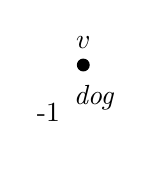
\begin{tikzpicture}
  [
    n/.style={circle,fill,draw,inner sep=1.5pt,node distance=1.5cm},
    aSniffing/.style={->, >=stealth, semithick, shorten <= 3pt, shorten >= 3pt},
  ]
 \node[n,label=above:$v$,label=below:{\relsize{-1}$\begin{array}{c}\nDog\\\ \end{array}$}] (a) {};
 \end{tikzpicture}}
 \end{picture}
&
\begin{picture}(55,50)
\put(0,0){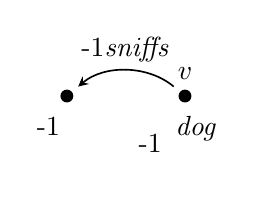
\begin{tikzpicture}
  [
    n/.style={circle,fill,draw,inner sep=1.5pt,node distance=1.5cm},
    aSniffing/.style={->, >=stealth, semithick, shorten <= 3pt, shorten >= 3pt},
  ]
 \node[n,label=above:,label=below:{\relsize{-1}$\begin{array}{c}\ \end{array}$}] (a) {};

 \node[n,label=above:$v$,label=below:{\relsize{-1}$\begin{array}{c}\nDog\\\ \end{array}$}, right of=a] (b) {};

 \draw [aSniffing,bend right=40] (b) to node[auto,swap]{\relsize{-1}$\aSniffing$} (a);

 \end{tikzpicture}}
 \end{picture}
&
\begin{picture}(70,50) \put(0,0){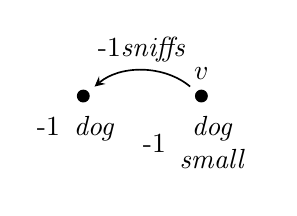
\begin{tikzpicture}
  [
    n/.style={circle,fill,draw,inner sep=1.5pt,node distance=1.5cm},
    aSniffing/.style={->, >=stealth, semithick, shorten <= 3pt, shorten >= 3pt},
  ]
 \node[n,label=above:,label=below:{\relsize{-1}$\begin{array}{c}\nDog\end{array}$}] (a) {};

 \node[n,label=above:$v$,label=below:{\relsize{-1}$\begin{array}{c}\nDog\\ \aSmall \end{array}$}, right of=a] (b) {};

 \draw [aSniffing,bend right=40] (b) to node[auto,swap]{\relsize{-1}$\aSniffing$} (a);

 \end{tikzpicture}}
 \end{picture}
&
\begin{picture}(77,50)
\put(0,0){\begin{tikzpicture}
  [
    n/.style={circle,fill,draw,inner sep=1.5pt,node distance=1.5cm},
    aSniffing/.style={->, >=stealth, semithick, shorten <= 3pt, shorten >= 3pt},
  ]
 \node[n,label=above:$v$,label=below:{\relsize{-1}$\begin{array}{c}\nDog\end{array}$}, right of=a] (b) {};
%
 \node[n,label=above:,label=below:{\relsize{-1}$\begin{array}{c}\nCat\\ \aSmall\end{array}$}, right of=b] (c) {};
%
 \draw [aSniffing,bend right=40] (c) to node[auto,swap]{\relsize{-1}$\aSniffing$} (b);
 \end{tikzpicture}}
 \end{picture}
% %
% \begin{picture}(77,50)
% \put(0,0){\begin{tikzpicture}
%   [
%     n/.style={circle,fill,draw,inner sep=1.5pt,node distance=1.5cm},
%     aSniffing/.style={->, >=stealth, semithick, shorten <= 3pt, shorten >= 3pt},
%   ]
%  \node[n,label=above:,label=below:{\relsize{-1}$\begin{array}{c}\end{array}$}] (a) {};
%
%  \node[n,label=above:$v$,label=below:{\relsize{-1}$\begin{array}{c}\end{array}$}, right of=a] (b) {};
%
%  \draw [aSniffing,loop left] (a) to node[above,xshift=-5pt]{\relsize{-1}$\aSniffing$} (a);
%
%  \draw [aSniffing,bend right=40] (b) to node[auto,swap]{\relsize{-1}$\aSniffing$} (a);
%  \end{tikzpicture}}
%  \end{picture}
\vspace{-.2cm}\ \\
(i)&(ii)&(iii)&(iv)
\end{tabular}
 \caption{Some connected subgraphs $(v,H)$ of scene $\+S$ in Figure~\ref{fig:cat-dog-1}.\label{fig:subgraphs}}
 \end{figure}

As an example, consider the relational model depicted in
Figure~\ref{fig:cat-dog-1} as a labeled graph $G$, and let us
discuss the pairs of nodes and connected subgraphs $(v,H)$ shown in
Figure~\ref{fig:subgraphs}. Clearly, (i) refers to the pair $(w,G)$
for any node $w\in\{a,b,d\}$; (ii) refers to $(w,G)$ for
$w\in\{b,d\}$; and both (iii) and (iv) uniquely refer to $(b,G)$. Notice
that (i)--(iv) can be respectively realized as ``{\em a dog}'',
``{\em a dog that sniffs something}'', ``{\em a small dog that
sniffs a dog}'' (cf. $\gamma_1$ in Table~\ref{tab:gammas}) % and ``{\em
% something that
% sniffs something else that sniffs itself}''.
and ``{\em the dog that is sniffed by a small cat}'' (cf.~$\gamma_4$ in
Table~\ref{tab:gammas}).


% For reasons of space we assume the reader is familiar with this
% algorithm and refer her to that article for further
% information.\fxnote{\tiny Intentemos depender lo menos posible del
% articulo de Krahmer.  En todo caso, dar una idea intuitiva del
% approach antes de decir esto.  Tenemos todavia una pagina. }



% \fxnote{\tiny Reescribir los siguientes dos parrafos. Decir algo como, 'once
% more we'll try to remain as close as possible to the algorithms of the original
% article and we will then start by pointing out the differences with the algorithms
% we presented in the previous section'}

It is important to emphasize that there is a substantial difference
between the algorithm presented in~\cite{Krahmer2003} and the one we discussed
in the previous sections:
%
% First note that scenes are encoded in that article in a slightly
% different way: there, graphs have only labels on edges, and
% non-relational attributes such as \emph{type} or \emph{color} are
% represented by loops (e.g., $\aSmall(a,a)$). % \fxnote{\tiny Aca decia
% `While our presentation is, arguably, conceptually cleaner, it
% forces us to treat the atomic and relational cases separately'. No
% hablemos de `our presenation' respecto de la de la seccion anterior.
% O ninguna o las dos son `our presentation'. }
%
while the input is a labeled graph $G$ and a target node $v$, the
output is, in this case (and unlike the definition of $\+L$-GRE problem
presented in \sect{technical} where the output is a {\em formula}), the cheapest (with
respect to some, previously specified cost function) connected
{\em subgraph} $H$ of $G$ which uniquely refers to $(v,G)$ if there is
such $H$, and $\bot$ otherwise.

We will not deal with cost functions here; it is enough to know
that a cost function is a monotonic function that assigns to each
subgraph of a scene graph a non-negative number which expresses the
goodness of a subgraph --e.g.\ in Figure~\ref{fig:subgraphs}, one
may tune the cost function so that (iii) is cheaper than (iv), and hence
(iii) will be preferred over (iv).
%By defining cost functions in
%different ways, \cite{Krahmer2003} shows that it is possible to mimic various algorithms for the
%generation of referring expressions known from the literature.

For reasons of space we will not introduce here the detailed algorithm proposed
in~\cite{Krahmer2003}. Roughly, it is a
straightforward branch and bound algorithm that systematically tries all
relevant subgraphs $H$ of $G$ by starting with the subgraph
containing only vertex $v$ and expanding it recursively by trying to
add edges from $G$ that are adjacent to the subgraph $H$ constructed
up to that point. In the terminology
of~\cite{Krahmer2003} a {\em distractor} is a node of $G$ different from
$v$ that is also referred by $H$.
The algorithm ensures that a subgraph uniquely refers to the
target $v$ when it has no distractors. Reached this point we
have a new candidate for the solution, but there can be other
cheaper solution so the search process continues until the
cheapest solution is detected. Cost functions are used to
guide the search process and to give preference to some solutions
over others.
% In the definition of~\cite{Krahmer2003}, $H$ is  such that every \emph{subgraph isomorphism}
% $f$ between $H$ and $G$ (i.e., every isomorphism between $H$
%  and a subgraph of $G$)
%  satisfies $f(u) = u$.
%

Here is the key link between the graph-based method
of~\cite{Krahmer2003} and our logical-oriented perspective: on
finite relational models, subgraph isomorphism corresponds to
\EPFOL-simulations, in the sense that given two nodes $u,v$ of
$G$, there is a subgraph isomorphic to $G$ via $f$, containing $u$ and
$v$, and such that $f(u)=v$ iff $u \simul{\+\EPFOL} v$.
%
Having made explicit this notion of sameness and, with it, the
logical language associated to it, we can proceed to generalize the
algorithm to make it work for other languages, and to adapt it in
order to output a formula instead of a graph. This is shown in
Algorithms~\ref{alg:makeRE} and~\ref{alg:find}.
%
\begin{center}\begin{minipage}[t]{5.1cm}%
\begin{algorithm}[H]\small
\SetKwFunction{makeRE}{makeRE$_\+L$}
\SetKwFunction{findGraph}{find$_\+L$}
\SetKwFunction{init}{init_$\+L$}
\SetKwFunction{buildF}{buildF$_\+L$}

\caption{\small \texttt{makeRE}$_\+L$($v$)}\label{alg:makeRE}

%$v_H$ := \emph{new node}\;

\SetKwInOut{Input}{input}\SetKwInOut{Output}{output}
\Input{an implicit finite $G=\tup{\Delta_G,\interp{\cdot}}$ and $v\in\Delta_G$}
\Output{an $\+L$-RE for $v$ in $G$ if there is one, or else $\bot$}
\BlankLine

\vspace{3.0pt}

\BlankLine

$H$ := $\tup{\cset{v},\emptyset}$\; $f$ := $\cset{v \mapsto v}$\;
$H'$ := \findGraph($v, \bot, H, f$)\;
\BlankLine
\Return{\buildF$(H',v)$}\;
\end{algorithm}
  \end{minipage}
\hspace{.05cm}
  \begin{minipage}[t]{6.8cm}%
\begin{algorithm}[H] \small
\SetKwFunction{findGraph}{find$_\+L$} \SetKwFunction{cost}{cost}
\SetKwFunction{matchGraph}{match$_\+L$}
\SetKwFunction{extendGraph}{extend$_\+L$}


\caption{\small \texttt{find}$_\+L$($v, \mathit{best},
H,f$)}\label{alg:find}

\If{$\mathit{best} \neq \bot \land \cost(\mathit{best}) \leq
\cost(H)$}{\Return $\mathit{best}$} $\mathit{distractors}$ :=
$\cset{n \mid n \in \Delta_G, n \neq v , v \simul{\+L} n}$\;
\If{$\mathit{distractors} = \emptyset$}{\Return $H$}
\ForEach{$\tup{H',f'} \in \extendGraph(H,f)$}{
  $I$ := \findGraph($v,\mathit{best},H', f'$)\;
  \If{$\mathit{best} = \bot \lor \cost(I) \leq \cost(\mathit{best})$}{$\mathit{best} := I$}
} \Return{$\mathit{best}$}\;
\end{algorithm}
  \end{minipage}%
\end{center}
%
These algorithms are parametric on $\+L$; to make them concrete, one
needs to provide appropriate versions of \instFun{buildF}{\+L} and
\instFun{extend}{\+L}. The former transforms the computed {\em
graph} which uniquely refers to the target $v$ into an $\+L$-RE {\em
formula} for $v$; the latter tells us how to extend $H$ at each step
of the main loop of Algorithm~\ref{alg:find}. Note that, unlike the
presentation of~\cite{Krahmer2003}, \instFun{makeRE}{\+L} computes
not only a graph $H$ but also an $\+L$-simulation $f$. %%
%
% \begin{algorithm}\small
% \SetKwFunction{makeRE}{makeRE$_\+L$}
% \SetKwFunction{findGraph}{find$_\+L$}
% \SetKwFunction{init}{init_$\+L$}
% \SetKwFunction{buildF}{buildF$_\+L$}
%
% \caption{\small \texttt{makeRE}$_\+L$($v$)}\label{alg:makeRE} $v_H$
% := \emph{new node}\; $\tup{H,f}$ :=
% $\tup{\tup{\cset{v_H},\emptyset,\emptyset}, \cset{v_H \mapsto v}}$\;
% $H'$ := \findGraph($v_H, \bot, H, f$)\;
% \Return{\buildF($H',v_H$)}
% \end{algorithm}
%
%
% \begin{algorithm} \small
% \SetKwFunction{findGraph}{find$_\+L$} \SetKwFunction{cost}{cost}
% \SetKwFunction{matchGraph}{match$_\+L$}
% \SetKwFunction{extendGraph}{extend$_\+L$}
%
%
% \caption{\small \texttt{findGraph}$_\+L$($v_H, \mathit{best}, H,f$)}
%
% \If{$\mathit{best} \neq \bot \land \cost(\mathit{best}) \leq
% \cost(H)$}{\Return $\mathit{best}$} $\mathit{distractors}$ :=
% $\cset{n \mid n \in \Delta_G \land n \neq v \land v_H \simul{\+L}
% n}$\; \If{$\mathit{distractors} = \emptyset$}{\Return $H$}
% \ForEach{$\tup{H',f'} \in \extendGraph(H,f)$}{
%   $I$ := \findGraph($v_H,\mathit{best},H', f'$)\;
%   \If{$\mathit{best} = \bot \lor \cost(I) \leq \cost(\mathit{best})$}{$\mathit{best} := I$}
% } \Return{$\mathit{best}$}
% \end{algorithm}
%
%
In order to make the discussion of the differences with the original
algorithm simpler, we analyze next the case $\+L=\EPFOL$ and $\+L=\EL$.

% \instFun{buildF}{\EPFOL}
% and \instFun{extend}{\EPFOL} in
% Algorithms~\ref{alg:build-form-epfol}
% and~\ref{alg:extend-epfol}.
%
%
\paragraph{The case of $\EPFOL$.} From the computed cheapest isomorphic
subgraph $H'$ one can easily build an \EPFOL-formula that uniquely
describes the target $v$, as is shown in
Algorithm~\ref{alg:build-form-epfol}. Observe that if
$\FOL$-simulations were used instead, we would have to include also
which unary and binary relations \emph{do not hold} in $H'$.
%
\begin{center}\begin{minipage}[t]{6.3cm}%
\begin{algorithm}[H]\small
\caption{\small
\texttt{buildF}$_\EPFOL(H',v)$}\label{alg:build-form-epfol}
\textbf{let}
$H' = \tup{\cset{a_1\ldots a_n}, \interp{\cdot}}$,$v=a_1$\;
%\tcp{let $v=a_1$}
$\gamma$ := $\displaystyle \bigwedge_{\mathclap{a_i \neq a_j}} (x_i
\not\approx x_j) \land \bigwedge_{\mathclap{(a_i,a_j) \in
\interp{r}}} r(x_i,x_j) \land \bigwedge_{\mathclap{a_i \in
\interp{p}}}p(x_i)$

\BlankLine
\vspace{2.2pt}
\Return{$\exists x_2\ldots \exists x_n . \gamma$}\;
\end{algorithm}
\end{minipage}
\hspace{.2cm}
\begin{minipage}[t]{5.2cm}
\begin{algorithm}[H]\small
\SetKwFunction{extendGraph}{extend$_\EPFOL$}

\caption{\small
\texttt{extend}$_\EPFOL(H,f)$}\label{alg:extend-epfol}

 $A$ := $\cset{H {+} p(u) \mid u \in \Delta_H, $

 \hfill $u \in \interp{p}_G  \setminus \interp{p}_H}$\;

 $B$ := $\cset{H {+} r(u,v) \mid u \in \Delta_H, $

 \hfill $\{(u,v),(v,u)\}\cap \interp{r}_G \setminus \interp{r}_H\not=\emptyset}$\;

 \Return{$(A \cup B) \times \cset{\mathit{id}}$}\;
\end{algorithm}
\end{minipage}
\end{center}
%
Regarding the function which extends the given graph in all possible
ways (Algorithm~\ref{alg:extend-epfol}), since $H$
 is a subgraph of $G$, $f$ is the
trivial identity function $\mathit{id(x)} = x$. We will see the need
for $f$ when discussing the case of less expressive logics like \EL.
In \instFun{extend}{\EPFOL} we follow the notation
of~\cite{Krahmer2003} and write, for a relational model
$G = \tup{\Delta,
\interp{\cdot}}$,  $G + p(u)$ to denote the model $\tup{\Delta
\cup \cset{u},\interp{\cdot}'}$ such that $\interp{p}' = \interp{p}
\cup \cset{u}$ and $\interp{q}' = \interp{q}$ when $q \neq p$.
Similarly, $G + r(u,v)$ denotes the model $\tup{\Delta \cup
\cset{u,v},\interp{\cdot}'}$ such that $\interp{r}' = \interp{r}
\cup \{(u,v)\}$ and $\interp{q}' = \interp{q}$ when $q \neq r$. It
is clear, then, that this function is returning all the
\emph{extensions} of $H$ by adding a missing attribute or relation
to $H$, just like is done in the original algorithm.

\paragraph{The case of $\EL$.}
Observe that \instFun{find}{\EL} uses an \EL-simulation, and any
\EPFOL-simulation is an \EL-simulation.
%
One could, in principle, just use \instFun{extend}{\EPFOL} also for
\EL. If we do this, the result of \instFun{find}{\EL} will be a
subgraph $H$ of $G$ such that for every \EL-simulation $\sim$, $u
\sim v$ iff $u = v$. The problem is that this subgraph $H$ may
contain cycles and, as it is well known, \EL (even \ALC) are
incapable to distinguish a cycle from its {\em
unraveling}\footnote{Informally, the unraveling of $G$, is a new
graph, whose points are paths of $G$ from a given starting node.
That is, transition sequences in $G$ are explicitly represented as
nodes in the unraveled model. See~\cite{BRV01} for a formal
definition.}. Hence, although subgraph isomorphism get along with
$\EPFOL$, it is too strong to deal with \EL.
%
%
% was observed in \sect{technical}, they cannot be
% distinguished using \EL.\fxnote{\tiny Esto no queda superclaro en la
% seccion anterior. La referencia es vaga. Vale la pena contar esto?}
% The upshot is that we might be unable to realize the outcome of such
% function.

A well-known result establishes that every relational model $\+M$ is
equivalent, with respect to \EL-formulas,\footnote{Actually, the
result holds even for \ALC-formulas.} to the unraveling of $\+M$.
That is, any model and its unraveling satisfy exactly the same \EL-formulas.
% \fxnote{\tiny tendriamos que introducir mejor
% (intuitvamente) que es el unraveling. Ademas de depender de Khramer
% estamos haciendo cambios usando cosas que no definimos bien.  Esta
% parte es muy dificil de leer.}
 Moreover, the unraveling of $\+M$ is
always a tree, and as we show in Algorithm~\ref{alg:build-form-el},
it is straightforward to extract a suitable \EL-formula from a tree.

Therefore, we need \instFun{extend}{\EL} to return all the possible
``extensions'' of $H$. Now ``extension'' does not mean to be a
subgraph of the original graph $G$ anymore. We do this
by either adding a new proposition or a new edge
that is present in the unraveling of $G$ but not in $H$. This is
shown in Algorithm~\ref{alg:extend-el}.
%
\begin{center}\begin{minipage}{5cm}%
\begin{algorithm}[H] \small
\SetKwFunction{buildF}{buildF$_\EL$} \caption{\small
\texttt{buildF}$_\EL(H',v)$}\label{alg:build-form-el} \mbox{{\bf
requires} $H'$ to be a tree}

$\gamma$ := $\cset{\exists r.\buildF(H',u) \mid$

\hfill$ (v,u) \in \interp{r}}$\;

\Return{$ (\bigwedge\gamma) \land (\bigwedge_{v \in
\interp{p}}p)$}\;
\end{algorithm}
\end{minipage}
\begin{minipage}{7cm}%
\begin{algorithm}[H]\small
\SetKwFunction{extendGraph}{extend$_\EL$} \caption{\small
\texttt{extend}$_\EL(H,f)$}\label{alg:extend-el}

$A$ :=\\
\ \ \ \ \  $\cset{\tup{H {+} p(u),f} \mid u \in \Delta_H, u \in
\interp{p}_G \setminus \interp{p}_H}$\; $B$ := $\emptyset$\;
\ForEach {$u \in \Delta_G$}{
  \ForEach{$u_H \in \Delta_H / (f(u_h),u) \in \interp{r}_G$}{
    \If{$\forall v : (u_H,v) \in \interp{r}_H \Rightarrow f(v) \neq u$}{
      $n$ := \emph{new node}\;
      $B$ := $B \ \cup $

      \hfill $\cset{\tup{H + r(u_H,n),f \cup \{n \mapsto u\}}}$\;
    }
  }
  }
  \Return{$A \cup B$}\;
\end{algorithm}
\end{minipage}
\end{center}
%
Observe that the behavior of \instFun{find}{\EL} is quite sensible
to the {\tt cost}  function employed. For instance, on cyclic models,
a {\tt cost} function that does not guarantee the unraveling is explored in a
breadth-first way may lead to non-termination (since
\instFun{find}{\EL} may loop exploring an infinite branch).

%It is also possible to use modal model-theoretical results to put a
%bound check that avoids generating an unraveling of infinite depth
%when there is no possible referring expression, but we will not go
%into the details for reasons of space.\fxnote{\tiny No tiene
%suficiente detalle para que se entienda.  Extender.}


% \begin{algorithm}\small
% \SetKwFunction{extendGraph}{extend$_\EL$}
% \caption{\small \texttt{extend}$_\EL(H,f)$}\label{alg:extend-el}
%
% $a$ :=  $\cset{\tup{H {+} p(u),f} \mid u \in \Delta_H, u \in \interp{p}_G {-} \interp{p}_H}$\;
% $b$ := $\emptyset$\;
% \ForEach {$u \in \Delta_G$}{
%   \ForEach{$u_H \in \Delta_H / (f(u_h),u) \in \interp{r}_G$}{
%     \If{$\forall v . ((u_H,v) \in \interp{r}_H \Rightarrow f(v) \neq u)$}{
%       $n$ := \emph{new node}\;
%       $b$ := $b \cup \cset{\tup{H + r(u_H,n),f[n \mapsto u]}}$\;
%     }
%   }
%   }
%   \Return{$a \cup b$}
% \end{algorithm}


As a final note on complexity, although the set of \EL-distractors
may be computed more efficiently than \EPFOL-distractors (since
\EL-distractors can be computed in polynomial time, and computing
\EPFOL-distractors seems to require a solution to the subgraph
isomorphism problem which NP-complete), we cannot conclude that
\instFun{find}{\EL} is more efficient than \instFun{find}{\EPFOL} in
general: the model built in the first case may be exponentially
larger --it is an unraveling, after all. We will come back to this
in~\sect{size}.


\section{Combinaci\'on de m\'etodos GRE}\label{sec:combining}

Una caracter\'istica atractiva de la formulaci\'on de la expresividad del problem GRE es que uno puede dise\~nar estrategias generales que combinan algoritmos L-GRE. Ilustramos esto con un ejemplo.
Los algoritmos basados en $\+L$-simulador de conjuntos como los de \sect{simulation} simult\'aneamente
calcular expresiones referenciales para cada objeto en el dominio, y hacer esto para
muchas l\'ogicas en tiempo polinomial. Esta es una propiedad interesante cuando uno anticipates la necesidad de referirse a un gran n\'umero de elementos. Sin embargo, esta familia
de algoritmos no es tan
flexible en cuanto a las preferencias de implementaci\'on como los que
introducido en ~\sect{krahmer} {aunque algunos
flexibilidad puede obtenerse mediante el uso de funci\'on de costo
ciones para la selecci\'on de u, v y w en el bucle principal del algoritmo 2 en lugar de las opciones no deterministas.
Hay una manera sencilla de obtener un algoritmo que es un compromiso entre
estas dos t\'ecnicas. Sea $A_1$ y $A_2$ dos procedimientos que resuelven el $\+L$-GRE
basado en las t\'ecnicas de \sect{simulation} y~\sect{krahmer}, respectivamente problema. Uno puede primero computar una $\+L$-RE para cada objeto posible utilizando $A_1$ y luego (con pereza) reemplazar el
RE calculada para $u$  con $A_2(u)$ cada vez que el ex no se ajusta a alguna
PREDE criterio definido. Esto es correcto, pero lo hacemos mejor, aprovechando la
clases de equivalencia obtuvieron utilizando $A_1$.

Desde que $A_1$ computa, para un modelo dado $\+M = \tup{\Delta,\interp{\cdot}}$, el conjunto
 $\simset(u)$ para todo $u \in \Delta$, uno puede construir en tiempo polinomial, usando la salida de $A_1$, el modelo $\+M_{\+L} = \tup{\cset{[u] \mid u \in \Delta}, \interp{\cdot}_{\+L}}$,
tal que:
$[u] = \cset{v \mid u \simul{\+L} v$ and $v \simul{\+L}
u}\quad \mbox{and}\quad \interp{r}_{\+L} = \cset{([u_1]\ldots [u_n])
\mid (u_1\ldots u_n) \in \interp{r}}$.
% $$
% \begin{array}{l@{\;=\;}l}
% \setlength{\abovedisplayskip}{0pt}%
% \setlength{\abovedisplayshortskip}{0pt}%
% [u] & \cset{v \mid u \simul{\+L} v \text{ and } v \simul{\+L} u}\\
% %\interp{p}_{\+L} &= \cset{[u] \mid u \in \interp{p}}\\
% \interp{r}_{\+L} & \cset{([u_1]\ldots [u_n]) \mid (u_1\ldots u_n) \in \interp{r}}
% \end{array}
% $$
$\+M_{\+L}$ es conocido como \emph{the $\+L$-minimization de $\+M$}. Por inducci\'on en $\gamma$ uno puede verificar que
$(u_1\ldots u_n) \in \interp{\gamma}$ iff $([u_1]\dots [u_n]) \in
\interp{\gamma}_{\+L}$ y esto implica que $\gamma$ es un $\+L$-RE
for $u$ in $\+M$ iff esto es un $\+L$-RE para $[u]$ in $\+M_{\+L}$.

Si $\+M$ tiene un gran n\'umero de elementos no distinguibles (usando $\+L$), entonces
 $\+M_{\+L}$ ser\'a mucho m\'as peque\~na que $\+M$. Desde que la  complejidad computational de
 $A_2$ depende del tama\~no de $\+M$, para escenas muy grandes, uno deberia computar en cambio
 $A_2([u])$.


%6 En el Tama\~no de las Expresiones referencia
%
%La fuerza expresiva de un lenguaje L determina si hay un L-RE para una
%elemento u. Tambi\'en en
%uye el tama\~no de la m\'as corta L-RE (cuando existen).
%Intuitivamente, con potencia m\'as expresiva podemos `ver 'm\'as? Cias y di
%por lo tanto tienen m\'as recursos a la mano para construir una f\'ormula m\'as breve.
%Una pregunta natural es, entonces, si podemos caracterizar el tama\~no relativo de
%la L-ER para un determinado L. Es decir, si podemos dar (ajustados) l\'imites superiores para el tama\~no
%de los m\'as cortos L-RE para los elementos de un modelo arbitrario M, como una funci\'on
%del tama\~no de M.
%Para el caso de una de las l\'ogicas m\'as expresivos considerados en este art\'iculo,
%FO?, la respuesta sigue de algoritmo makeREFO? en x4. De hecho, si un FO?-
%RE existe, que se calcula buildFFO? de un modelo H que no es m\'as grande que
%el modelo de entrada. Es f\'acil ver que esta f\'ormula es lineal en el tama\~no de H y,
%Por lo tanto, el tama\~no de cualquier FO?-RE es O (#? + #jj? jj). No es dif\'icil ver que
%este l\'imite superior es v\'alido para FO-ER tambi\'en.
%Uno est\'a tentado a concluir de Teorema 2 que el tama\~no de la EL- m\'as corto
%RE es O (#?? #jj? Jj), pero hay una trampa. Teorema 2 asume que las f\'ormulas
%se representa como un DAG y garantiza que este DAG es polinomio en
%el tama\~no del modelo de entrada. Uno puede reconstruir f\'acilmente (el \'arbol de sintaxis) la
%f\'ormula de la DAG, pero esto, en principio, puede conducir a un soplado exponencial
%up {el resultado ser\'a una f\'ormula exponencialmente m\'as grande, pero compuesta de s\'olo unas
%n\'umero polinomio de di? subf\'ormulas Erent. Como muestra el siguiente ejemplo,
%de hecho es posible obtener un EL-f\'ormula que es exponencialmente m\'as grande cuando
%la ampliaci\'on de la representaci\'on DAG generada por el algoritmo 2.
%Ejemplo 1. Considere una lengua con s\'olo un binario relaci\'on r, y dejar M =
%�marido?; jj? JJI d\'onde? = F1; 2; :::; ng y (i; j) 2 jjrjj i? i <j. Algoritmo 2 inicializa
%F (j) => para todo j 2?. Supongamos las siguientes opciones en la ejecuci\'on: Para
%i = 1; :::; n ? 1, iterar n ? i veces recogiendo v = w = n ? i + 1 y sucesivamente
%u = n ? i; :::; 1. Se puede demostrar que cada vez que una f\'ormula F (j) se actualiza, se
%cambia de 'a' ^ 9r: 'y por lo tanto, se duplica su tama\~no. SDesde F (1) se actualiza
%n ? 1 muchas veces, el tama\~no de F (1) es mayor que 2n.
%
%
%La gran EL-RE del Ejemplo 1 se debe a una desafortunada (no determinista)
%elecci\'on de los elementos. Ejemplo 2 muestra que otra ejecuci\'on conduce a una cuadr\'atica
%RE (notar la m\'as corta es lineal: (9r) (n?1):>).
%Ejemplo 2. Supongamos ahora que en el primer n?1 iteraciones elegimos sucesivamente
%v = w = n ? i y u = v ? 1 para i = 0::: n ? 2. Puede verse que para una mayor
%opciones convenientes, F (1) es de tama\~no O (n2).
%Pero, �es siempre posible obtener un EL-RE de tama\~no polinomio en el tama\~no
%del modelo de entrada, cuando representamos una f\'ormula como una cadena, y no como un DAG?
%En [12] se muestra que la respuesta es 'no': para L 2 Falc; EL; EL + g, menor
%con destino a la longitud de la L-RE es exponencial en el tama\~no de la model11 de entrada,
%y este l\'imite inferior es estrecho.
%7 Conclusiones
%La fase de determinaci\'on del contenido durante la generaci\'on de expresiones que se refieren
%es identi las que se destinar\'an `propiedades" para referirse a un objeto de destino o conjunto
%de los objetos. Lo que se considera como un `propiedad 'es especificado en di? Maneras Erent por
%cada uno de los muchos algoritmos para la determinaci\'on del contenido existente en la literatura.
%En este art\'iculo, nos proponemos que este problema puede ser abordado por decidir
%cuando dos elementos deben ser considerados a ser igual, es decir, decidiendo qu\'e
%poder discriminatorio que desea utilizar. Formalmente, el que poder discriminatorio
%que desee utilizar en un caso particular puede ser especificado sint\'acticamente por elegir un
%en particular lenguaje formal o sem\'antico, por la elecci\'on de una noci\'on adecuada de
%simulaci\'on. Es irrelevante si elegimos RST lenguaje (y obtener el
%noci\'on asociada de la simulaci\'on despu\'es), o viceversa.
%Sostenemos que tiene tanto a la mano es extremadamente \'util. Obviamente, la
%lenguaje formal vendr\'a a mano como lenguaje de representaci\'on para que la salida
%el problema de determinaci\'on de contenido. Pero quiz\'as lo m\'as importante, una vez que
%han fijado la expresividad que queremos usar, podemos confiar en el modelo te\'orico
%resultados de nir la noci\'on adecuada de identidad que subyace en cada lengua, que
%indica lo que puede y no se puede decir (como ya comentamos en x2). Por otra parte, podemos
%transferir los resultados generales de los campos bien desarrollados de la l\'ogica computacional y
%la teor\'ia de grafos como veremos en x3 y x4, donde generalizamos algoritmos conocidos
%en familias de algoritmos GRE para di? Erent lenguajes l\'ogicos.
%Una noci\'on expl\'icita de expresividad tambi\'en proporciona una interfaz m\'as limpia, ya sea
%entre los m\'odulos de determinaci\'on y realizaci\'on de contenidos superficie o entre
%dos colaboradoras m\'odulos de determinaci\'on de contenido. Un ejemplo de este \'ultimo era
%expuesto en x5.
%Como una l\'inea de futuro de la investigaci\'on, uno puede querer evitar apegarse a un fijo L pero
%en cambio favorecer un enfoque gradual en el que cuenta con una m\'as expresiva
%idioma L1 se utilizan s\'olo cuando L0 no es suficiente para distinguir cierto elemento.
%11 M\'as precisamente, no se encuentran en los modelos nite G1; G2; ::: Tal que para cada i, el tama\~no de
%Gi es lineal en i pero el tama\~no de la RE m\'inimo para alg\'un elemento en Gi est\'a limitada
%desde abajo por una funci\'on exponencial que es en i.




